% Paquets généraux
\documentclass[a4paper,12pt,titlepage,twoside]{article}
\usepackage[T1]{fontenc}
\usepackage[utf8]{inputenc}
\usepackage[french]{babel}
\usepackage{subcaption}
\addto\captionsfrench{%
  \renewcommand{\tablename}{Tableau}%
}
\usepackage[gen]{eurosym}
%\usepackage[dvips]{graphicx}
\usepackage{minted}
\usepackage{fancyhdr}
\usepackage{pdfpages} 
\usepackage{multido}
\usepackage{hyperref}
\usepackage{textcomp}
\usepackage{schemabloc}
%\usepackage[bitstream-charter]{mathdesign}
\usepackage{array}
\newcolumntype{P}[1]{>{\centering\arraybackslash}p{#1}}
\usepackage[shortlabels]{enumitem}
\usepackage[framemethod=TikZ]{mdframed}

\newcommand{\id}{71}
\newcommand{\nom}{Théorie des mécanismes}
\newcommand{\sequence}{04}
\newcommand{\nomsequence}{Liaisons entre les solides}
\newcommand{\num}{02}
\newcommand{\type}{KH}
\newcommand{\descrip}{Liaisons équivalentes, hyperstatisme, liaisons en série et en parallèle, théorie des graphes}
\newcommand{\competences}{B2-12: Proposer une modélisation des liaisons avec leurs caractéristiques géométriques. \\ &  B2-13: Proposer un modèle cinématique paramétré à partir d'un système réel, d'une maquette numérique ou d'u \\ &  B2-17: Simplifier un modèle de mécanisme. \\ &  B2-18: Modifier un modèle pour le rendre isostatique. \\ &  C1-04: Proposer une démarche permettant d'obtenir une loi entrée-sortie géométrique.  \\ &  C2-05: Caractériser le mouvement d'un repère par rapport à un autre repère. \\ &  C2-06: Déterminer les relations entre les grandeurs géométriques ou cinématiques. }
\newcommand{\nbcomp}{7}
\newcommand{\systemes}{}
\newcommand{\systemesnum}{}
\newcommand{\systemessansaccent}{}
\newcommand{\ilot}{2}
\newcommand{\ilotstr}{02}
\newcommand{\dossierilot}{\detokenize{Ilot_02 }}

%\usepackage{style}
\usepackage{bodegraph}
\usepackage{rpcinematik}
\usepackage[locale = FR]{siunitx}
\usepackage{caption}
\newcommand{\institute}{Lycée Dorian}

\usepackage{listings}
\usepackage{fancyvrb}
\usepackage{color}
\usepackage{xcolor}
\usepackage{colortbl}
\usepackage{helvet}
\usepackage[frenchmath]{newtxsf} % for sans serif symbols
\renewcommand{\familydefault}{\sfdefault}
%\usepackage{amsfonts}
%\usepackage{amsmath}
%\usepackage{lmodern}
\usepackage{mathastext}
%\usepackage{xspace}
\usepackage{varioref}
\usepackage{tabularx}
%\usepackage{floatflt}
\usepackage{graphics}
\usepackage{wrapfig}
\usepackage{textcomp}
\usepackage{tikz,tkz-tab}
\usepackage[european resistor, european voltage, european current]{circuitikz}
\usepackage{wrapfig}
\usepackage{gensymb}
\usepackage[percent]{overpic}
\usetikzlibrary{babel}
\usepackage{ifthen}
\usepackage{cancel}
\usepackage{etoolbox}
\usepackage{multirow}
%\usepackage{boxedminipage}
\definecolor{gris25}{gray}{0.75}
\definecolor{bleu}{RGB}{18,33,98}
\definecolor{bleuf}{RGB}{42,94,171}
\definecolor{bleuc}{RGB}{231,239,247}
\definecolor{bleum}{RGB}{160,195,226}
\definecolor{rougef}{RGB}{185,18,27}
\definecolor{rougec}{RGB}{255,188,204}%255,230,231
\definecolor{vertf}{RGB}{103,126,82}
\definecolor{vertc}{RGB}{220,255,191}
\definecolor{forestgreen}{rgb}{0.13,0.54,0.13}
\definecolor{blcr}{rgb}{0.59,0.69,0.84}
\definecolor{blfr}{rgb}{0.32,0.51,0.75}
\definecolor{orfr}{rgb}{0.90,0.42,0.15}
\definecolor{orcr}{rgb}{0.90,0.65,0.50}
\definecolor{orangef}{rgb}{0.659,0.269,0.072}
\definecolor{orange}{rgb}{0.58,0.35,0.063}
\definecolor{orangec}{rgb}{0.43,0.32,0.25}
\definecolor{rcorrect}{rgb}{0.6,0,0}
\definecolor{sequence}{rgb}{0.75,0.75,0.75}
\definecolor{competences}{rgb}{0.61,0.73,0.35}
\definecolor{rose}{HTML}{ff00ff}
\definecolor{grisf}{HTML}{222222}
\definecolor{grisc}{HTML}{636363}
\definecolor{normal}{HTML}{4087c4}
\definecolor{info}{HTML}{5bc0de}
\definecolor{success}{RGB}{92,184,92}
\definecolor{warning}{RGB}{240,173,78}
\definecolor{danger}{RGB}{217,83,79}
\hypersetup{                    % parametrage des hyperliens
    colorlinks=true,                % colorise les liens
    breaklinks=true,                % permet les retours à la ligne pour les liens trop longs
    urlcolor= blfr,                 % couleur des hyperliens
    linkcolor= orange,                % couleur des liens internes aux documents (index, figures, tableaux, equations,...)
    citecolor= forestgreen                % couleur des liens vers les references bibliographiques
    }

\newcolumntype{M}[1]{>{\centering\arraybackslash}m{#1}}
\definecolor{codegreen}{rgb}{0,0.6,0}
\definecolor{codegray}{rgb}{0.5,0.5,0.5}
\definecolor{codepurple}{rgb}{0.58,0,0.82}
\definecolor{backcolour}{rgb}{0.95,0.95,0.92}

\lstdefinestyle{mystyle}{
    backgroundcolor=\color{backcolour},   
    commentstyle=\color{codegreen},
    keywordstyle=\color{magenta},
    numberstyle=\tiny\color{codegray},
    stringstyle=\color{codepurple},
    basicstyle=\ttfamily\footnotesize,
    breakatwhitespace=false,         
    breaklines=true,                 
    captionpos=b,                    
    keepspaces=true,                 
    numbers=left,                    
    numbersep=5pt,                  
    showspaces=false,                
    showstringspaces=false,
    showtabs=false,                  
    tabsize=2
}

\lstset{style=mystyle}

% Mise en page
\pagestyle{fancy}

\setlength{\hoffset}{-18pt}
\setlength{\oddsidemargin}{0pt} 	% Marge gauche sur pages impaire2s
\setlength{\evensidemargin}{0pt} 	% Marge gauche sur pages paires
\setlength{\marginparwidth}{00pt} 	% Largeur de note dans la marge
\setlength{\headwidth}{481pt} 	 	% Largeur de la zone de tête (17cm)
\setlength{\textwidth}{481pt} 	 	% Largeu\textbf{r de la zone de texte (17cm)
\setlength{\voffset}{-18pt} 		% Bon pour DOS
\setlength{\marginparsep}{7pt}	 	% Séparation de la marge
\setlength{\topmargin}{-30pt} 		% Pas de marge en haut
\setlength{\headheight}{55pt} 		% Haut de page
\setlength{\headsep}{20pt} 		% Entre le haut de page et le texte
\setlength{\footskip}{30pt} 		% Bas de\textbf{ page + séparation
\setlength{\textheight}{700pt} 		% Hauteur de l'icone zone de texte (25cm)
\setlength\fboxrule{1 pt}
\renewcommand{\baselinestretch}{1}
\setcounter{tocdepth}{1}
\newcommand{\cadre}[2]
{\fbox{
  \begin{minipage}{#1\linewidth}
   \begin{center}
    #2\\
   \end{center}
  \end{minipage}
 }
}

\newcommand{\repon}[1]
{
~\ \\
\begin{tabular}{|m{\linewidth}|}
 \hline
\multido{}{#1}{\\ \hline}
\end{tabular}
}


\newcommand{\objectif}[1]{
\mdfsetup{%
frametitle={%
\tikz[baseline=(current bounding box.east),outer sep=0pt]
\node[anchor=east,rectangle,fill=bleum]
{\strut Objectif~};}}
\mdfsetup{innertopmargin=10pt,linecolor=bleum,%
linewidth=2pt,topline=true,%
frametitleaboveskip=\dimexpr-\ht\strutbox\relax
}
\begin{mdframed}[]\relax%
#1
\end{mdframed}}


\newcounter{num_quest} \setcounter{num_quest}{0}
\newcounter{num_rep} \setcounter{num_rep}{0}
\newcounter{num_cor} \setcounter{num_cor}{0}

\newcommand{\feuilleDR}[1]{
	\begin{tikzpicture}
		\draw[gray!30](0,0)grid[step=0.5cm](\linewidth,#1);
	\end{tikzpicture}
}

%\newcommand{\question}[1]{\refstepcounter{num_quest}\par
%~\ \\ \parbox[t][][t]{0.15\linewidth}{\textbf{Question \arabic{num_quest}}}\parbox[t][][t]{0.85\linewidth}{#1\label{q\the\value{num_quest}}}\par
%}

\newcommand{\question}[1]{\refstepcounter{num_quest}\par
~\ \\ \textbf{Question \arabic{num_quest} : }#1\label{q\the\value{num_quest}}\par
}

\newcommand{\posetafigure}[3]{
\begin{figure}[ht!]
 \begin{center}
  \includegraphics[width=#2\linewidth]{img/#1}
 \end{center}
 \caption{\label{#1} #3}
\end{figure}}

\newcommand{\goforum}{
\begin{figure}

\end{figure}
\begin{center}
 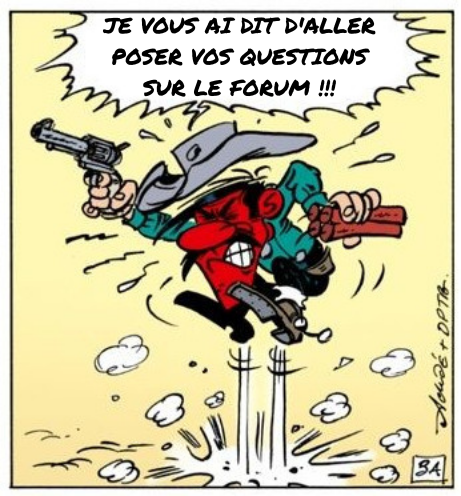
\includegraphics[width=0.7\linewidth]{../../../img/go_forum}
\end{center}
\label{go_forum}
\caption{J'pète les plombs}
\end{figure}}

\newcommand{\reponse}[4][1]
{\noindent
\parbox{\textwidth}{
\rule{\linewidth}{.5pt}\\
\textbf{Question\ifthenelse{#1>1}{s}{} \multido{}{#1}{%
\refstepcounter{num_rep}\ref{q\the\value{num_rep}} }:} ~\ \\
\ifdef{\public}{#3 \ifthenelse{#2>0}{~\ \\ 	\feuilleDR{#2}}}{#4}
}}

\newcommand{\cor}
{\refstepcounter{num_cor}
\noindent
\rule{\linewidth}{.5pt}
\textbf{Question \arabic{num_cor}:} \\
}

\newcommand{\finsujet}
{
    \begin{center}
    \Large{FIN}
    \end{center}

    \cleardoublepage

    \ifdef{\public}{\pagestyle{docreponse}}{\pagestyle{correction}}

    \ifdef{\public}{
        \begin{tikzpicture} 
            \draw (0,0) rectangle (2,2);
            \draw (0,0) -- (2,2);
            \draw (1.5,0.5) node {\large 20};
            \draw (2.5,0) rectangle (16,2);
            \draw (4.5,1.7) node {\large Commentaires:};
        \end{tikzpicture}
    }
    ~\ \\
}


%\newcommand{\repcarre}[2]
%{
%~\ \\
%\begin{tikzpicture}
%\draw [fill=white] (0,0) rectangle +(\linewidth,#1);
%\node[align=left] at (1.1,#2-0.3) {\textbf{Question #1:}};
%\end{tikzpicture}
%}

\newcommand{\titre}[1]
{\begin{center}
\cadre{0.8}{\huge #1} 
\end{center}
}


%Définition des torseurs :
\newcommand{\torseur}[2]{\left\{\mathcal{#1}_{#2} \right\}}
\newcommand{\torseurh}[3]{\left\{\genfrac{}{}{0pt}{0}{#1}{#2}\right\}_{#3}}
\newcommand{\torseurv}[8]{\left\{
\begin{matrix}
#1 & #4 \\ #2 & #5 \\ #3 &#6
\end{matrix}
\right\}_{{#7},{#8}}}

%Définition des torseurs :
%\newcommand{\torseur}[2]{\left \{\mbox{\relsize{2}{$\mathcal {#1}$}\relsize{-2}}\phantom{}_{\mbox{\scriptsize $#2$}} \right \}}
%\newcommand{\torseurh}[3]{\left\{\genfrac{}{}{0pt}{0}{#1}{#2}\right\}_{#3}}
%\newcommand{\torseurv}[8]{
%\left\{\begin{array}{@{}c|c@{}} #1 & #4 \\ #2 & #5 \\ #3 & #6 \end{array} \right\}_{#7,#8}
%}
\newcommand{\derivee}[2]{\left.\dfrac{\d #1}{\d t}\right|_{#2}}
\newcommand{\tripleint}{\int\!\!\!\!\!\int\!\!\!\!\!\int}

% Notation cinématique et statique
\newcommand{\cinematique}[2]{\mbox{#1}/\mbox{#2}}
\newcommand{\statique}[2]{\mbox{#1}\rightarrow\mbox{#2}}
\newcommand{\moment}[3]{\vv {#1}_{\scriptsize{#3}}(#2)}
\newcommand{\resultante}[2]{\vv {#1}_{\scriptsize{#2}}}


%Commande de base
\newcommand{\jo}{\left(j\omega\right)} % j \omega dans l'analyse fréquentielle
\newcommand{\tl}{\xrightarrow{\mathcal{L}}} % transformée de laplace sur fleche
\newcommand{\tli}{\xrightarrow{\mathcal{L}^{-1}}} % transformée inverse de laplace sur fleche
\renewcommand{\d}[1][]{\mathrm{d#1}}
\newcommand{\dd}[1][]{\mathrm{d#1}}
\newcommand{\vect}[2]{{#1}\wedge{#2}}
\newcommand{\base}[3]{(\vec #1,\vec #2,\vec #3)}
\newcommand{\vectbase}[4]{{\vphantom{\left| \begin{matrix}
#1\\#2\\#3 \end{matrix} \right|}}_{#4}{\left| \begin{matrix}
#1\\#2\\#3 \end{matrix} \right.}}
%Pour avoir les paragraphes sous la forme I, II, III
\renewcommand{\thesection}{\Roman{section}}
\setcounter{secnumdepth}{3}
\renewcommand{\Frlabelitemii}{$\bullet$}

% En tête et pied de page
\lhead{\nom}
\rhead{
\includegraphics[width=2cm]{../../../img/logo}}
\lfoot{\auteurun,\ \auteurdeux}
\cfoot{Page \thepage}

\fancypagestyle{docreponse}{%
  \fancyhf{}
  \fancyhead[LO]{NOM Prénom: .............................}
  \rhead{
\includegraphics[width=2cm]{../../../img/logo}\hspace{2pt}}
  \ifdef{\auteurdeux}{\lfoot{\auteurun,\ \auteurdeux}}{\lfoot{\auteurun}}
  \rfoot{\nom}
  \lfoot{Document réponse}
  \cfoot{Page \thepage}
   }

\fancypagestyle{correction}{%
  \fancyhf{}
  \lhead{\colorbox{danger}{\begin{minipage}{0.65\paperwidth} \textcolor{white}{\textbf{Correction}} \end{minipage}} }
  \rhead{
\includegraphics[width=2cm]{../../../img/logo}}
  \lfoot{Renaud Costadoat, Françoise Puig}
  \rfoot{\colorbox{danger}{\begin{minipage}{0.4\paperwidth} \begin{flushright}\textcolor{white}{\textbf{Correction}}\end{flushright} \end{minipage}} }}

\fancypagestyle{correctioninfo}{%
  \fancyhf{}
  \lhead{\colorbox{danger}{\begin{minipage}{0.65\paperwidth} \textcolor{white}{\textbf{Correction}} \end{minipage}} }
  \rhead{
\includegraphics[width=2cm]{../../../img/logo}}
  \lfoot{Renaud Costadoat, Juliette Genzmer}
  \rfoot{\colorbox{danger}{\begin{minipage}{0.6\paperwidth} \begin{flushright}\textcolor{white}{\textbf{Correction}}\end{flushright} \end{minipage}} }}

\renewcommand{\footrulewidth}{0.4pt}

\usepackage{eso-pic}
\newcommand{\BackgroundPic}{%
\put(0,0){%
\parbox[b][\paperheight]{\paperwidth}{%
\vfill
\begin{center}
\hspace{0.5cm}\vspace{0.5cm}
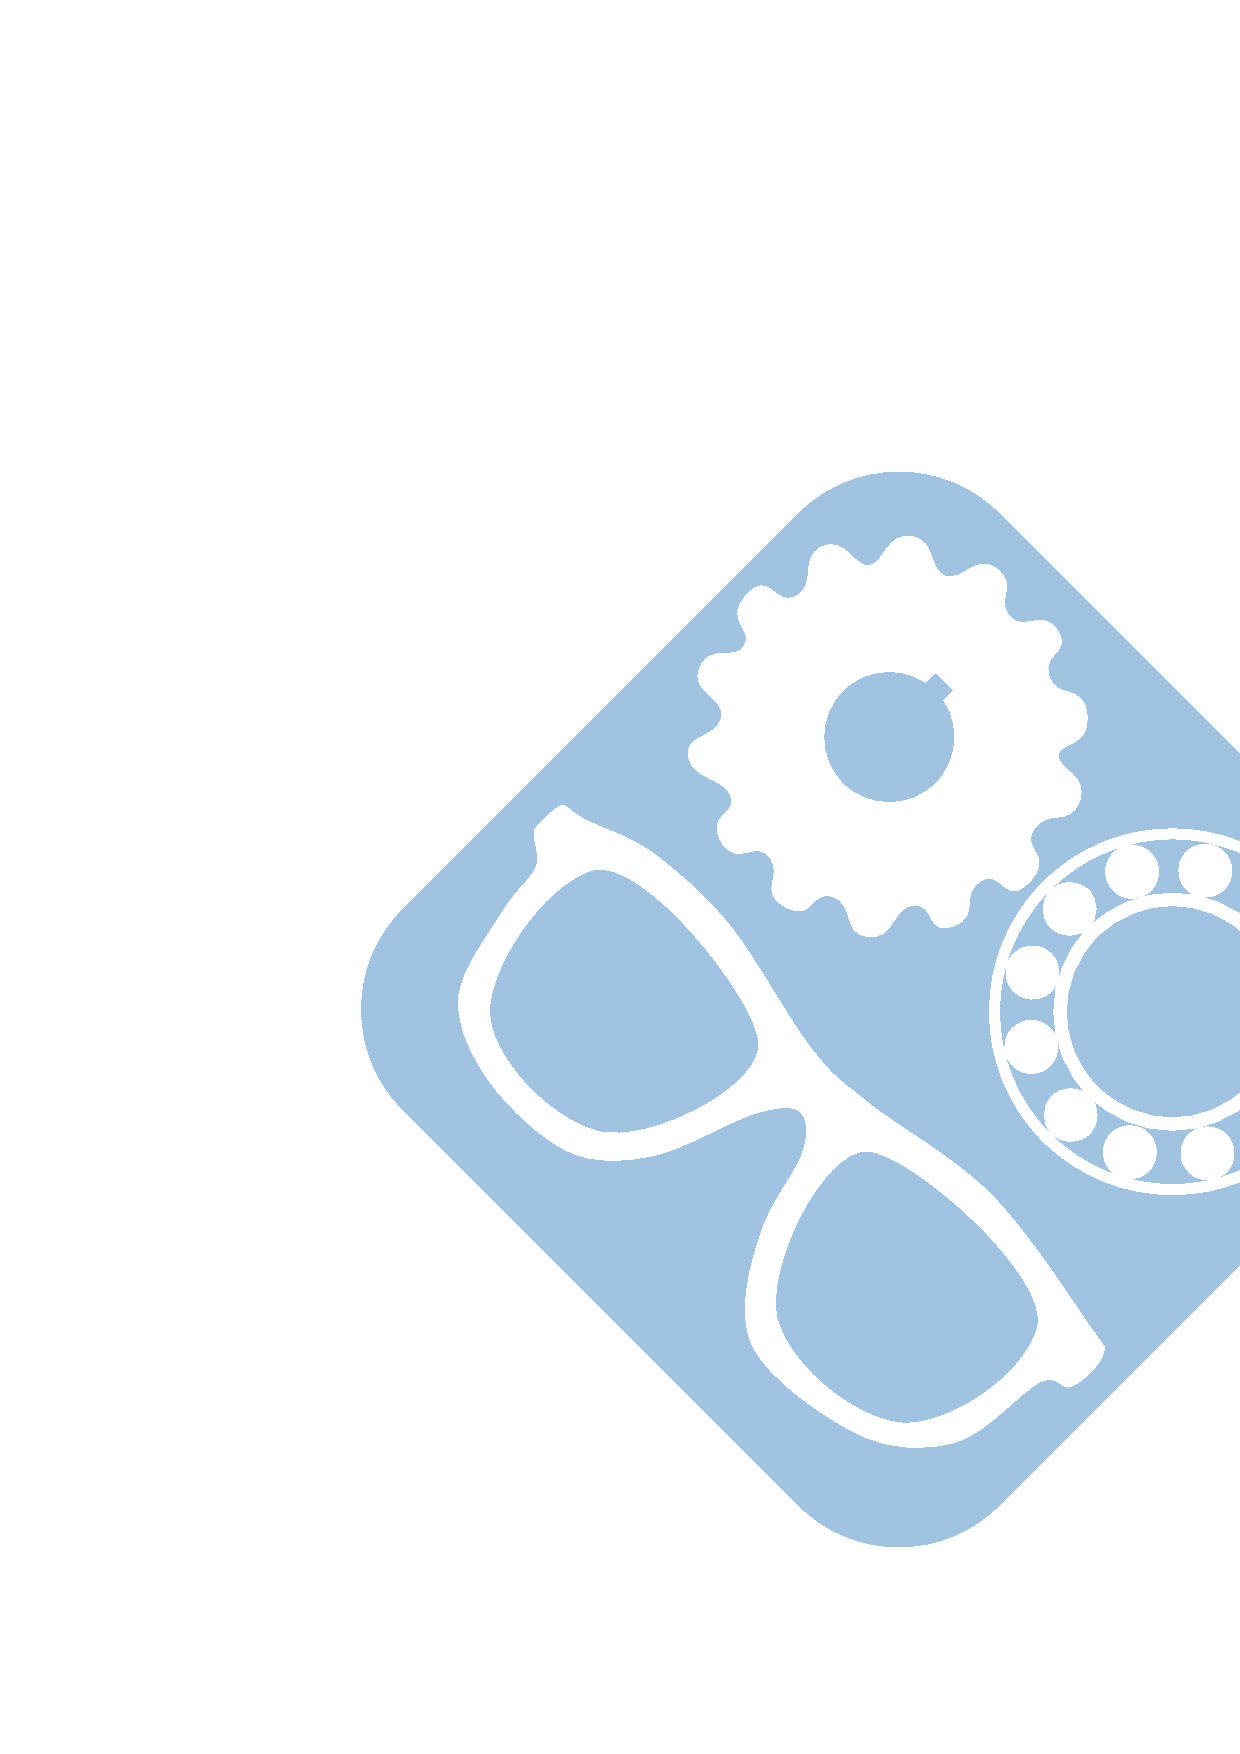
\includegraphics[width=\paperwidth,height=\paperheight,%
keepaspectratio]{../../../img/fond3}%
\end{center}
\vfill
}}}

\newcommand{\BackgroundPicdeux}{%
\put(25,-30){%
\parbox[b][\paperheight]{\paperwidth}{%
\vfill
\begin{center}
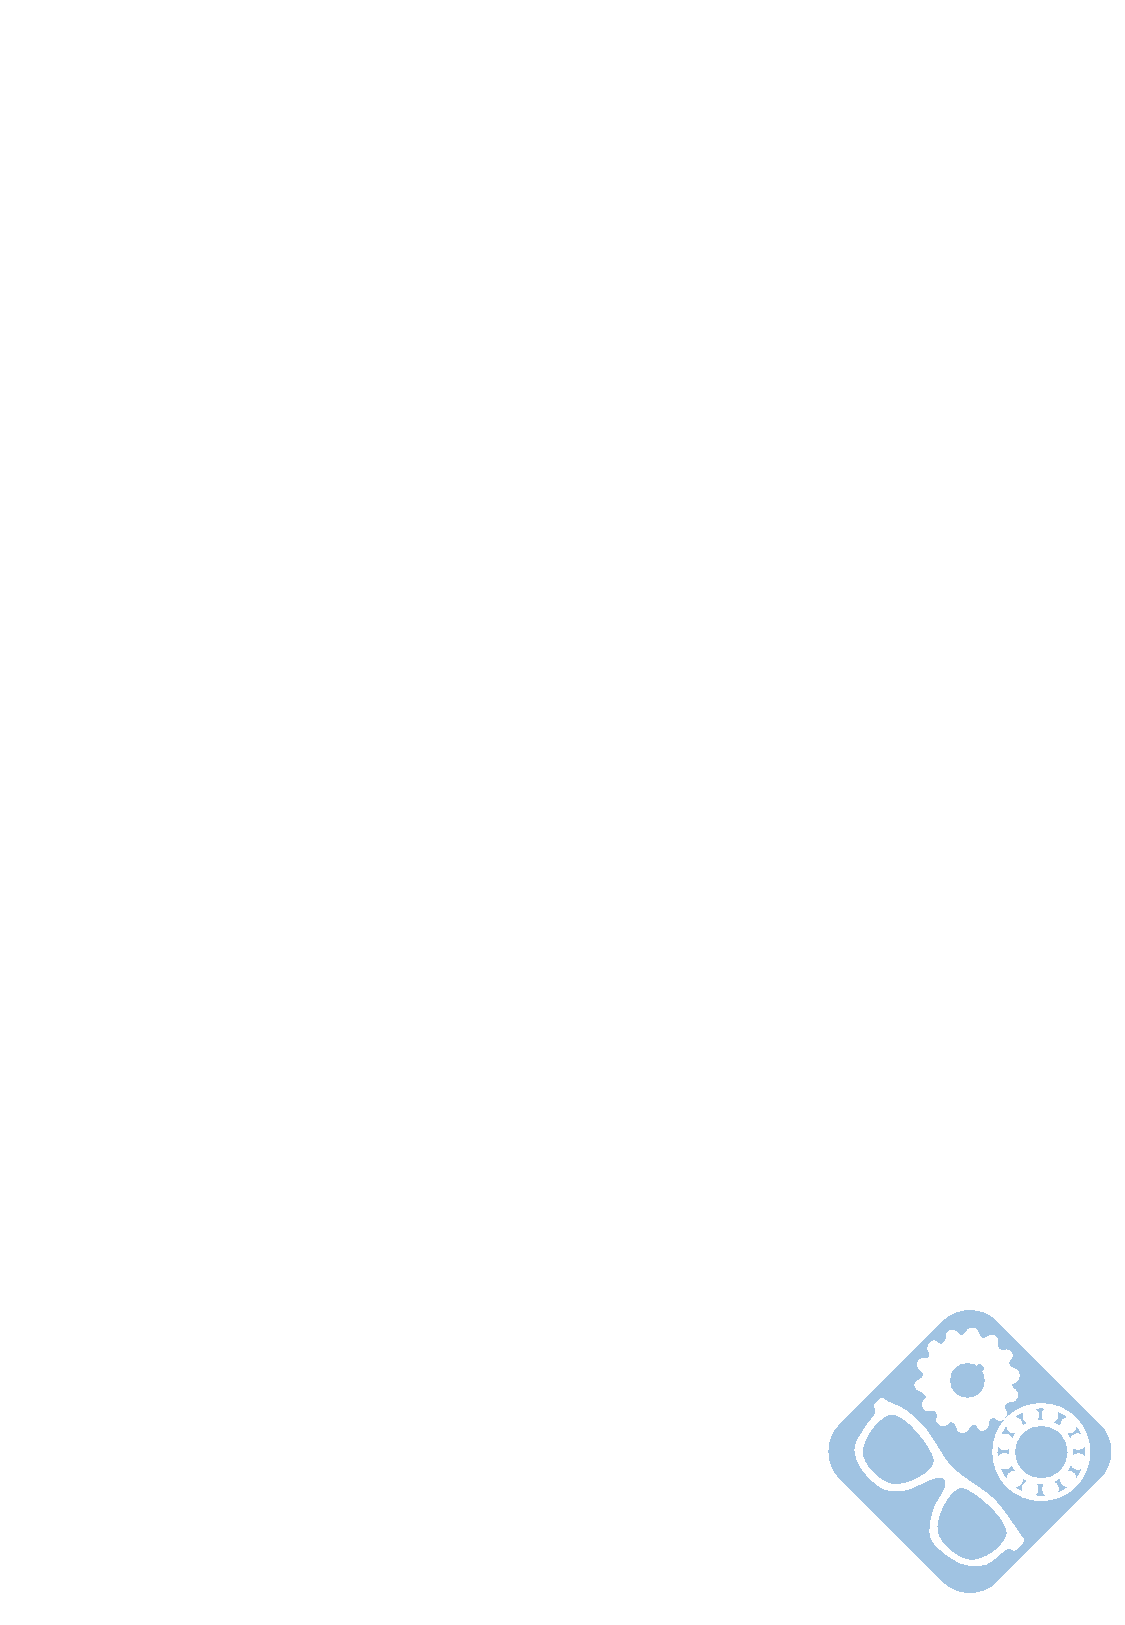
\includegraphics[width=\paperwidth,height=\paperheight,%
keepaspectratio]{../../../img/fond4}%
\end{center}
\vfill
}}}

\begin{document}

\pagestyle{empty}

\AddToShipoutPicture*{\BackgroundPic}


\includegraphics[width=2cm]{../../../img/logo}

\Huge{DS \numero - \sujet}

\vspace{1cm}

\ifdef{\prive}{\begin{center}\colorbox{danger}{\Huge{Avec Correction}}\end{center}}{}

\begin{center}
\centering\huge{PTSI}
\end{center}

\vspace{2cm}


\begin{center}
\centering\Large{\jour}
\end{center}

\vspace{2cm}

\normalsize

\tableofcontents

\newpage

\AddToShipoutPicture{\BackgroundPicdeux}

\pagestyle{fancy}

\begin{center}
\Huge \sujet
\end{center}


\normalsize


\section{Présentation du téléphérique Vanoise Express (10 min)}

\subsection{Mise en situation}

\begin{figure}[!h]
\centering
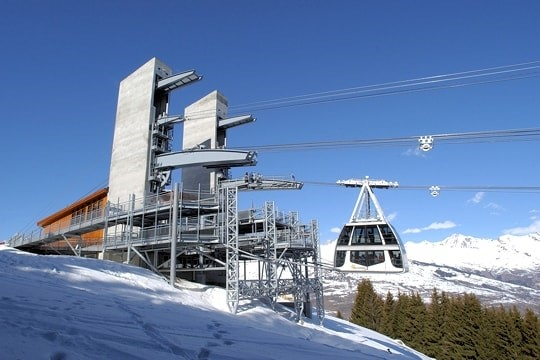
\includegraphics[width=0.8\linewidth]{img/fig01}
\caption{Téléphérique Vanoise Express}
\label{fig01}
\end{figure}

\begin{wrapfigure}{r}{50mm}
	\vspace{-20pt}
	\centering 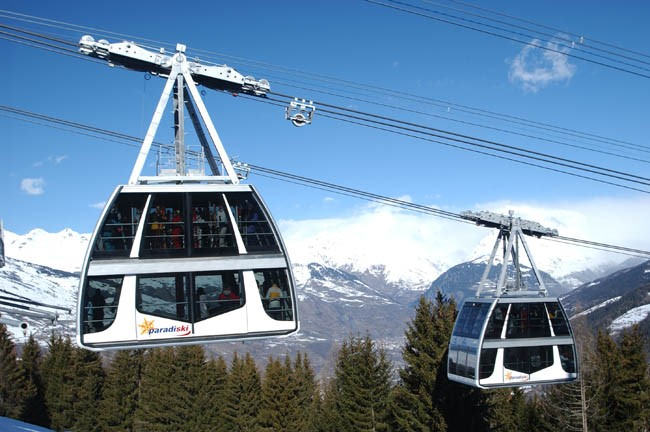
\includegraphics[width=0.9\linewidth]{img/fig02}
	\caption{Cabines se déplaçant sur une ligne}
	\label{fig02}
\end{wrapfigure}

Noël 2003, le téléphérique Vanoise Express relie enfin les domaines skiables de La Plagne et Les Arcs, donnant naissance à paradiski, un domaine skiable de 425 km, le troisième plus grand de France.
	Le Vanoise Express est une prouesse technologique de 16.5 millions \euro. C'est le plus grand téléphérique de ce type jamais construit au monde. Il est réalisé par la société POMAGALSKI. C'est un téléphérique sans pylônes, d'une seule portée de gare à gare, ce qui permet de diminuer l'impact sur l'environnement et de préserver la beauté du paysage. L'utilisation de cabines à deux étages permet de réduire le volume des cabines et des gares, améliorant l'esthétique de l'ensemble (voir photo \ref{fig02}).
	La solution retenue est constituée de deux lignes parallèles portant chacune une seule cabine. Contrairement à la plupart des téléphériques, \textbf{les deux lignes sont entièrement indépendantes}, ce qui signifie qu'une cabine n'est pas le contrepoids de l'autre. Ainsi, en cas de problème sur une cabine, la liaison entre les deux stations n'est pas interrompue. 

\textbf{L'étude qui suit ne porte que sur une seule ligne et donc une seule cabine}.
Le schéma de principe d'une ligne est donné en annexe 1. La capacité de chaque cabine est de 200 personnes. La puissance installée de 1060 kW par cabine autorise un débit maximum de 1000 personnes à l'heure dans chaque sens et par cabine. Chaque ligne est composée principalement de deux câbles porteurs (rails) et d'un câble tracteur (voir photo \ref{fig03}).

\newpage

\begin{figure}[!h]
\centering
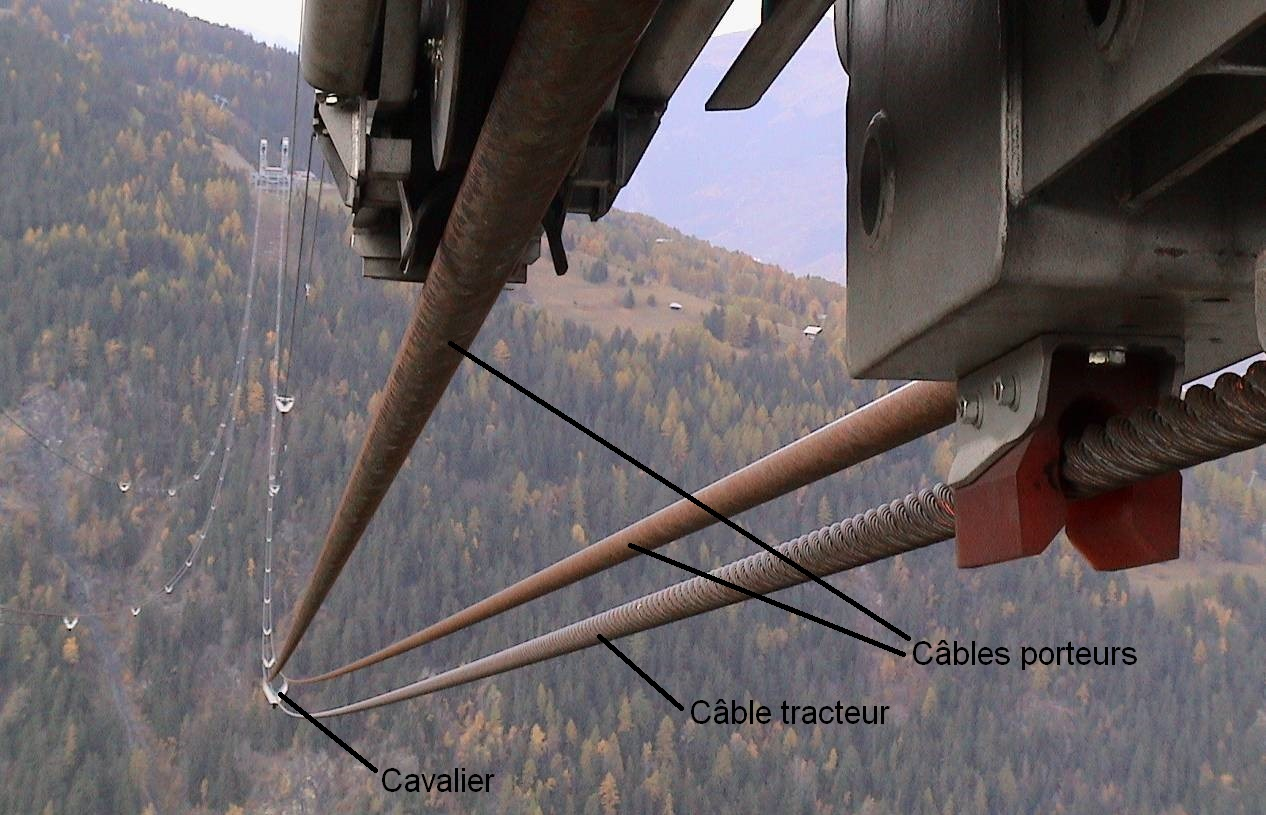
\includegraphics[width=0.6\linewidth]{img/fig03}
\caption{Vue d'une ligne du téléphérique}
\label{fig03}
\end{figure}

\textbf{Le câble tracteur $\Phi 45mm$}

\begin{wrapfigure}{r}{50mm}
	\vspace{-20pt}
	\centering 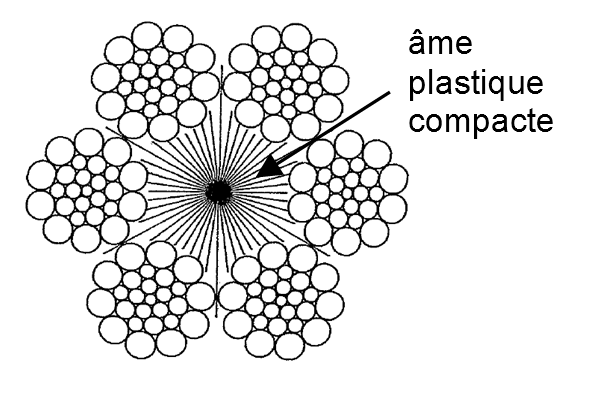
\includegraphics[width=0.9\linewidth]{img/fig04}
	\caption{Câble tracteur $\Phi45$, tension de rupture : $1430kN$}
	\label{fig04}
\end{wrapfigure}

Cet unique câble assure la transmission du mouvement depuis la poulie motrice ($\Phi D=4m$ en gare des Arcs) vers la cabine. Il est dévié par 5 poulies de déviation $\Phi d=3,8m$. Son âme plastique lui permet de s'enrouler facilement autour des poulies. Un contrepoids d'une masse $Mc=35$ tonnes en gare de La Plagne lui permet d'être toujours tendu. Cela permet de retenir ou de tirer la cabine pour voyager dans les deux sens de circulation. D'une masse $m=29$ tonnes, ce câble est guidé et porté tout le long du trajet par 50 petites poulies dont 32 sont montées sur des cavaliers. Il ne peut donc pas se tendre sous l'effet de son propre poids.
\\ ~\ \\
\textbf{Les deux câbles porteurs $\Phi 75mm$}

\begin{wrapfigure}{r}{50mm}
	\vspace{-20pt}
	\centering 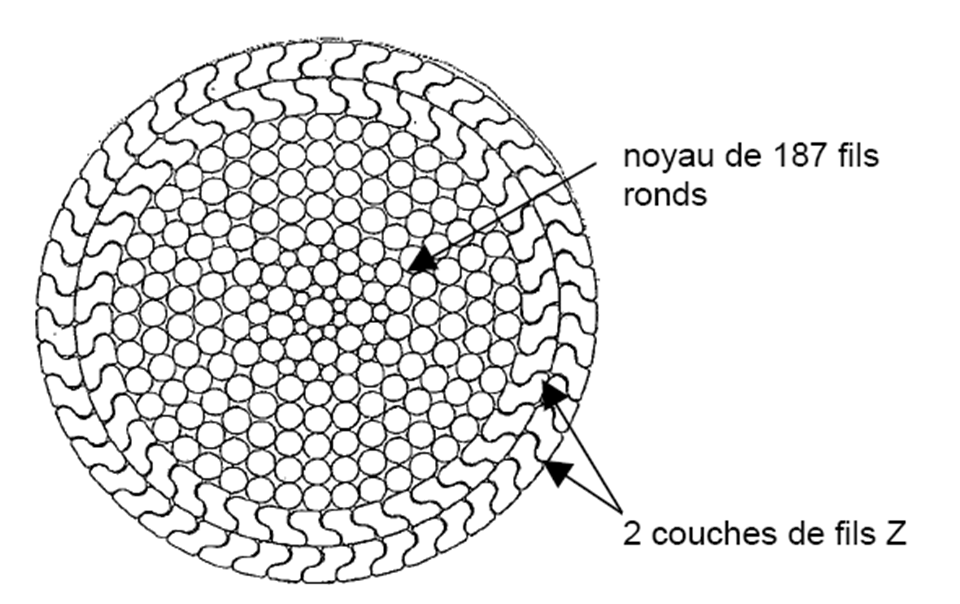
\includegraphics[width=0.9\linewidth]{img/fig05}
	\caption{Câble porteur $\Phi75$, tension de rupture : $6006kN$}
	\label{fig05}
\end{wrapfigure}

Leur fonction est de guider et porter le câble tracteur et la cabine (dont la masse maximum est M=29 tonnes). La cabine se déplace donc comme un wagon sur ces deux câbles tendus à $1300kN$ entre les deux gares. Ils sont de véritables rails, qui survolent la vallée à 380 m au dessus du sol. D'une masse respective de 55 tonnes, ils ne peuvent pas être horizontaux. Le trajet d'une gare à l'autre commence donc par une forte descente, suivi d'une montée de même pente (on néglige la différence d'altitude entre les deux gares).
\\ ~\ \\
\textbf{Les deux câbles porteurs $\Phi 42mm$}

\begin{wrapfigure}{r}{50mm}
	\vspace{-20pt}
	\centering 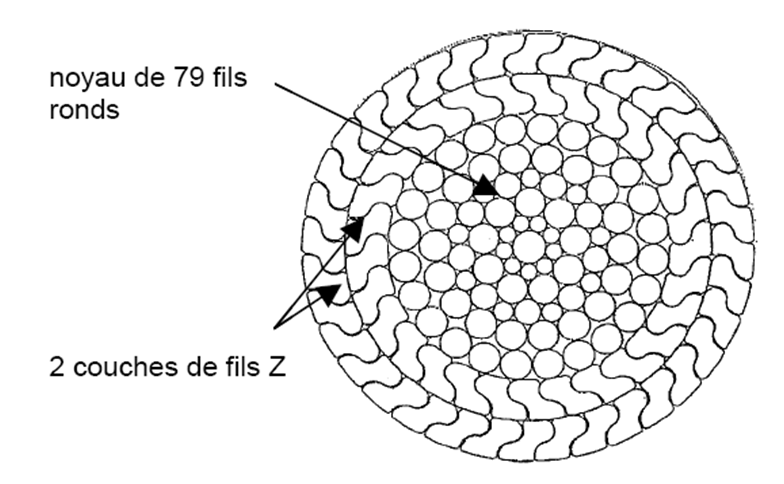
\includegraphics[width=0.9\linewidth]{img/fig06}
	\caption{Câble porteur	 $\Phi42$, tension de rupture : $2014kN$}
	\label{fig06}
\end{wrapfigure}

Tendus à $560kN$, ils soutiennent 16 cavaliers. Chacun guide en rotation une petite poulie dont la fonction est de porter le câble tracteur lors de son retour vers la poulie motrice.
\\ ~\ \\ ~\ \\ ~\ \\
\newpage

\begin{figure}[!h]
\centering
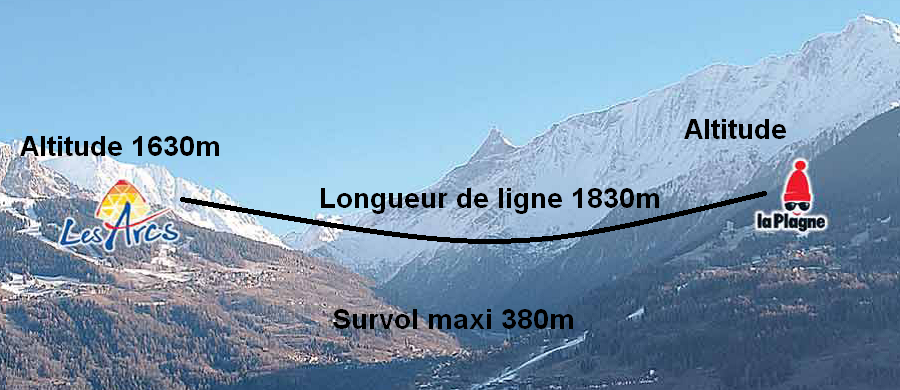
\includegraphics[width=0.6\linewidth]{img/fig07}
\caption{Vue de la vallée à survoler}
\label{fig07}
\end{figure}

\section{Description SysMl du téléphérique (5 min)}

\begin{figure}[!h]
\begin{minipage}{0.45\linewidth}
\centering
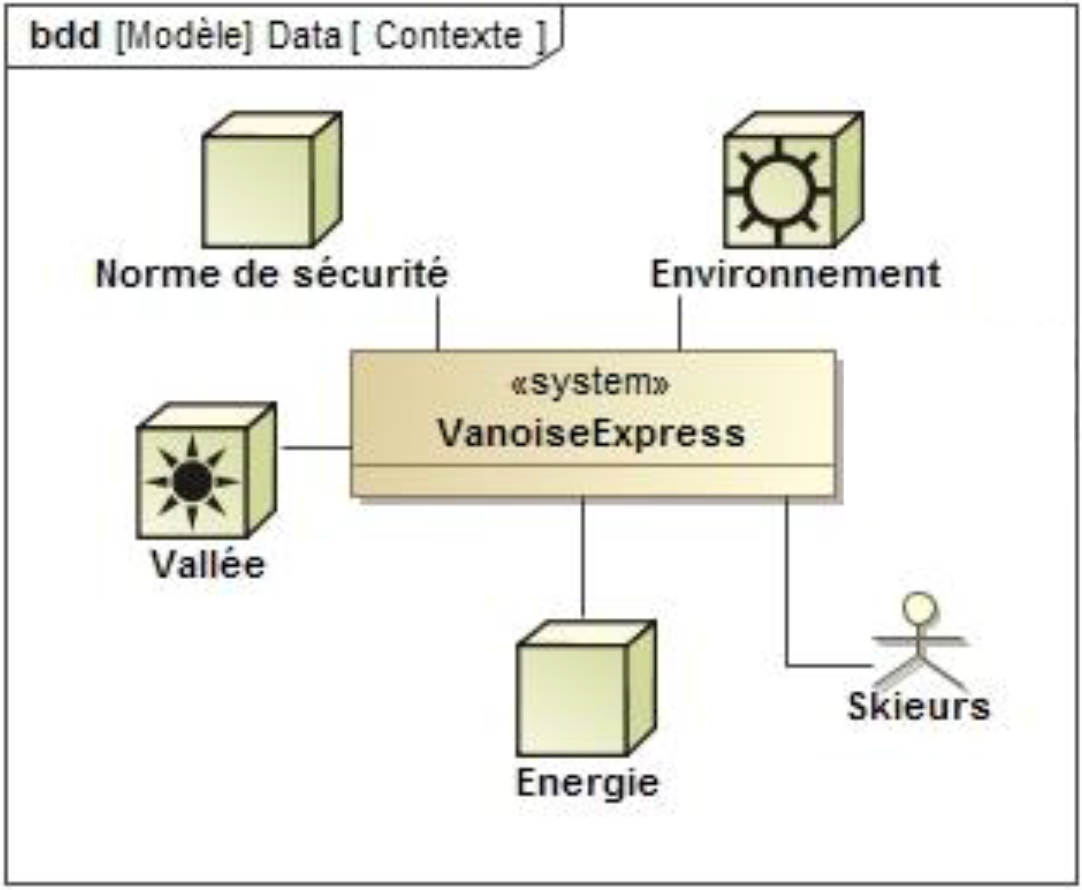
\includegraphics[width=0.8\linewidth]{img/fig08}
\caption{Diagramme de contexte partiel}
\label{fig08}
\end{minipage}\hfill
\begin{minipage}{0.45\linewidth}
\centering
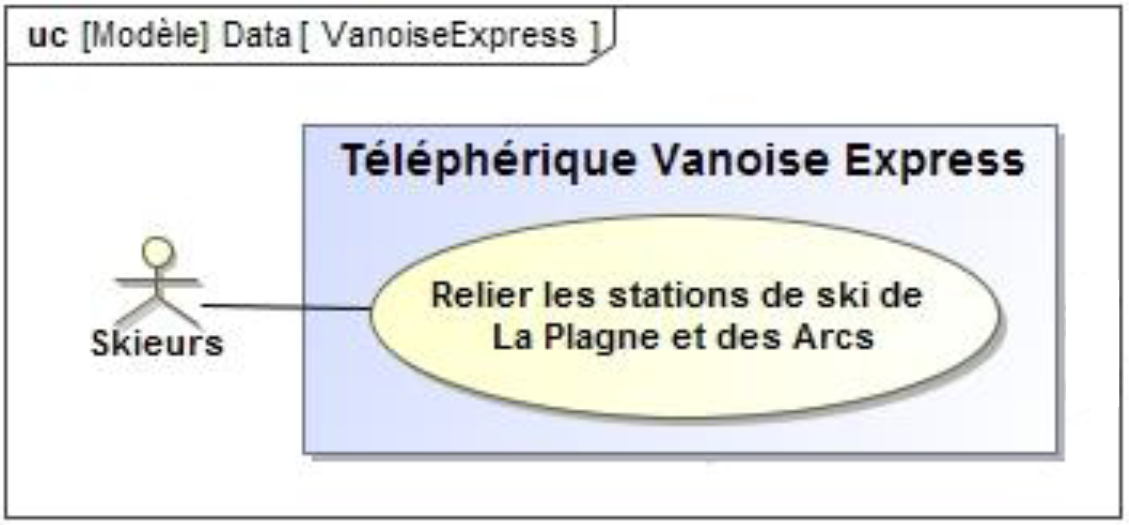
\includegraphics[width=0.8\linewidth]{img/fig09}
\caption{Diagramme de cas d'utilisation}
\label{fig09}
\end{minipage}
\end{figure}

\begin{figure}[!h]
\centering
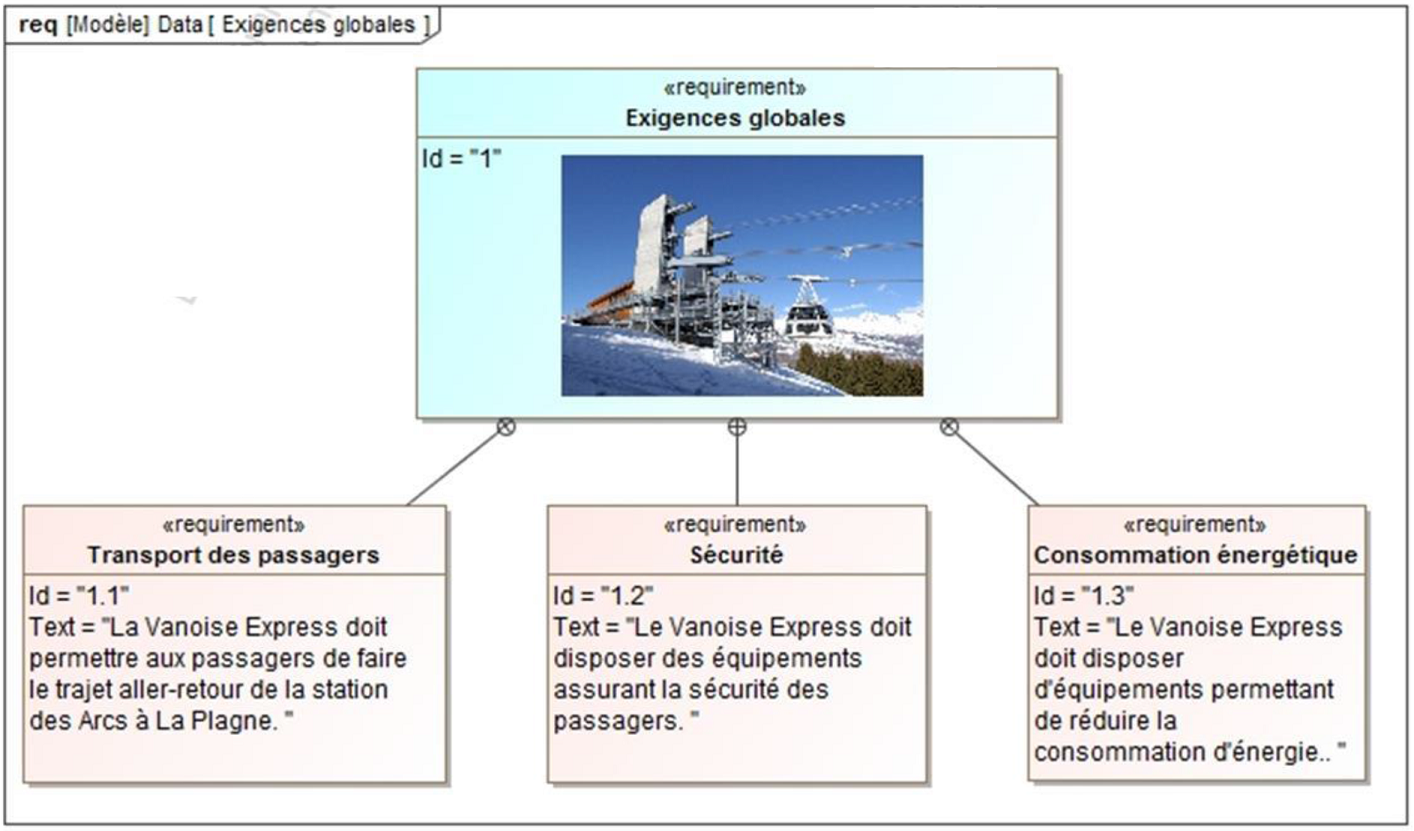
\includegraphics[width=0.8\linewidth]{img/fig10}
\caption{Diagramme des exigences globales}
\label{fig10}
\end{figure}

On peut montrer que l'on obtiendra un débit de 1000 passagers par heure dans chaque sens et par ligne si la durée du trajet est égale à 4 minutes. En effet, en considérant un temps de chargement-déchargement des cabines de 2 minutes, il faut donc 6 minutes pour transporter 200 personnes d'un côté à l'autre de la vallée, soit un aller retour en 12 minutes et donc un débit de 1000 personnes par heure dans chaque sens.

\begin{figure}[!h]
\centering
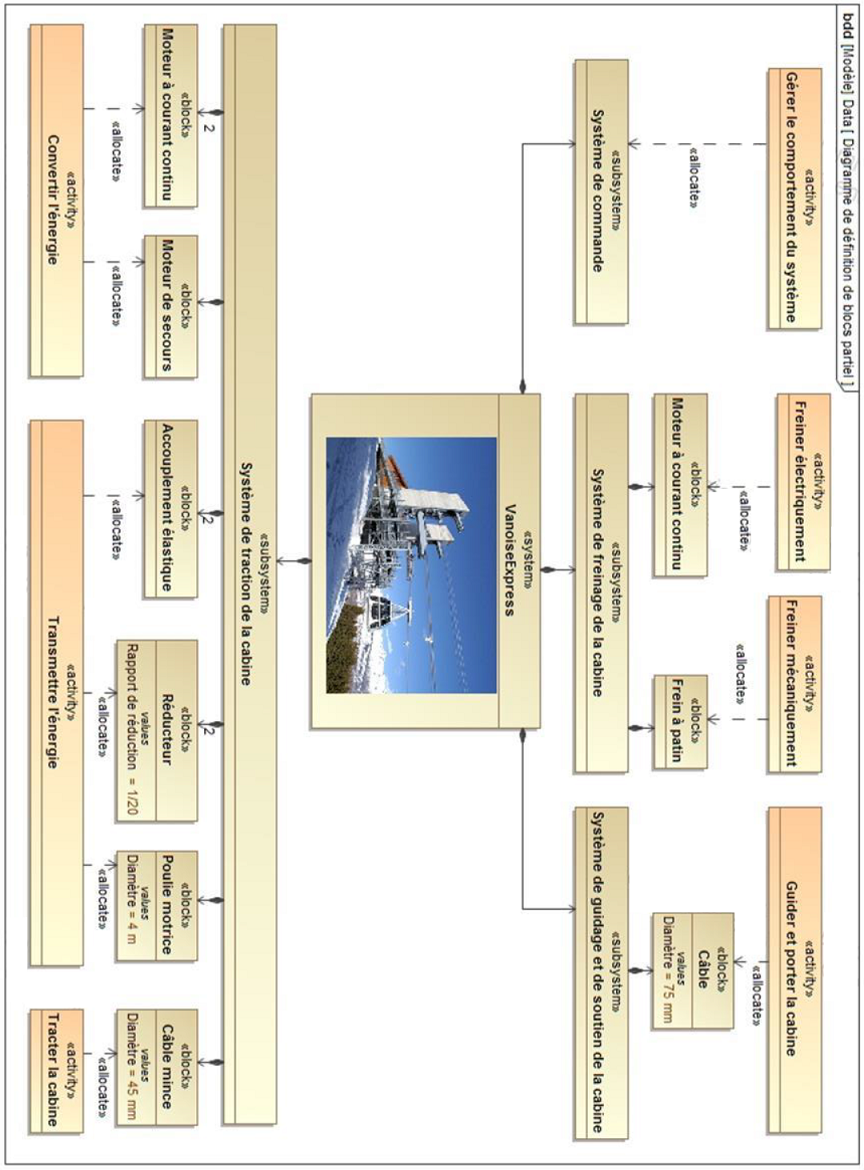
\includegraphics[width=0.9\linewidth]{img/fig11}
\caption{Diagramme de définition de bloc}
\label{fig11}
\end{figure}

\begin{figure}[!h]
\centering
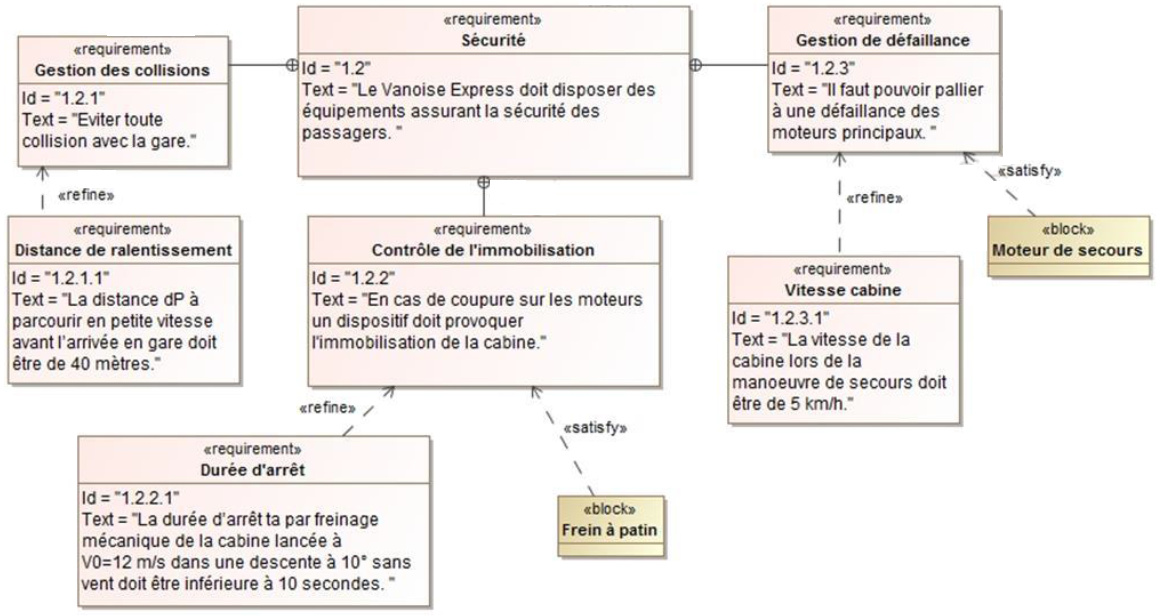
\includegraphics[width=0.75\linewidth]{img/fig12}
\caption{Exigence 1.2}
\label{fig12}
\end{figure}

\begin{figure}[!h]
\centering
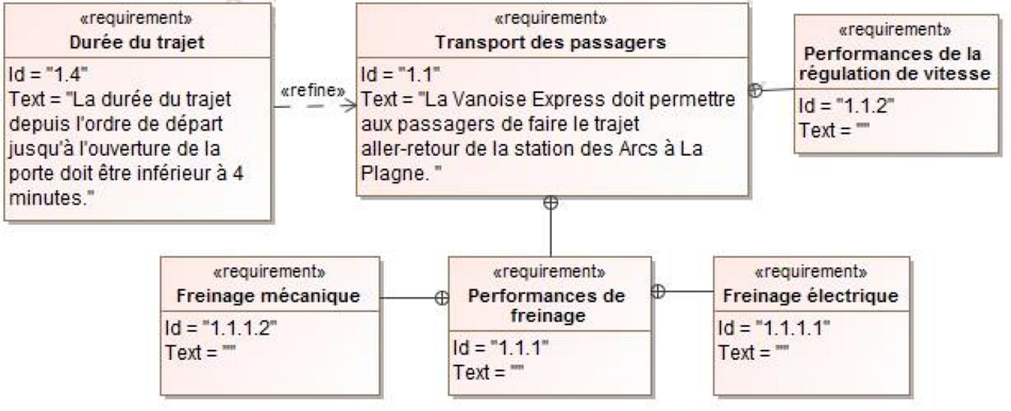
\includegraphics[width=0.75\linewidth]{img/fig13}
\caption{Exigence 1.1}
\label{fig13}
\end{figure}

\begin{figure}[!h]
\centering
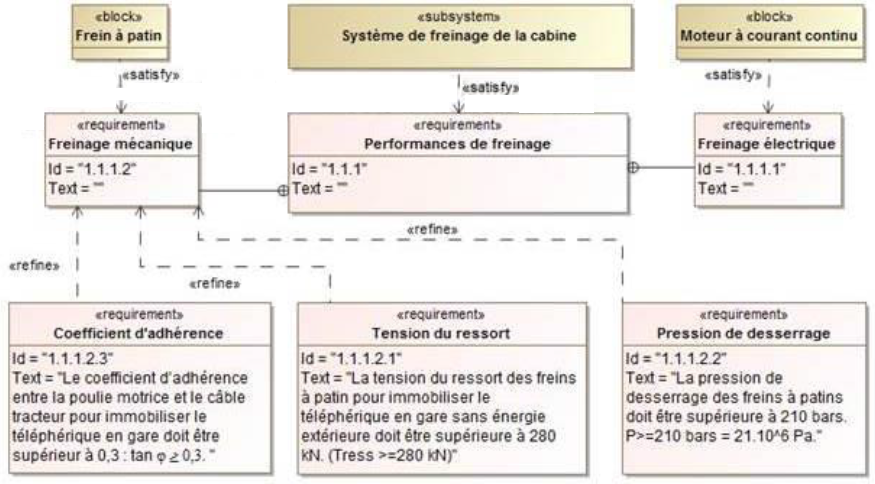
\includegraphics[width=0.75\linewidth]{img/fig14}
\caption{Exigence 1.1.1}
\label{fig14}
\end{figure}

\begin{figure}[!h]
\centering
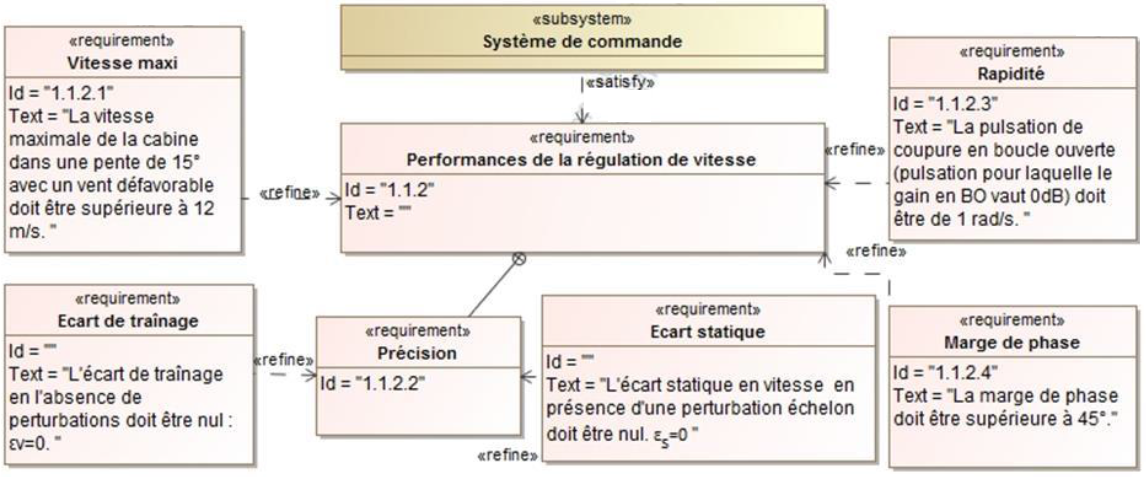
\includegraphics[width=0.9\linewidth]{img/fig15}
\caption{Exigence 1.1.2}
\label{fig15}
\end{figure}

\begin{figure}[!h]
\centering
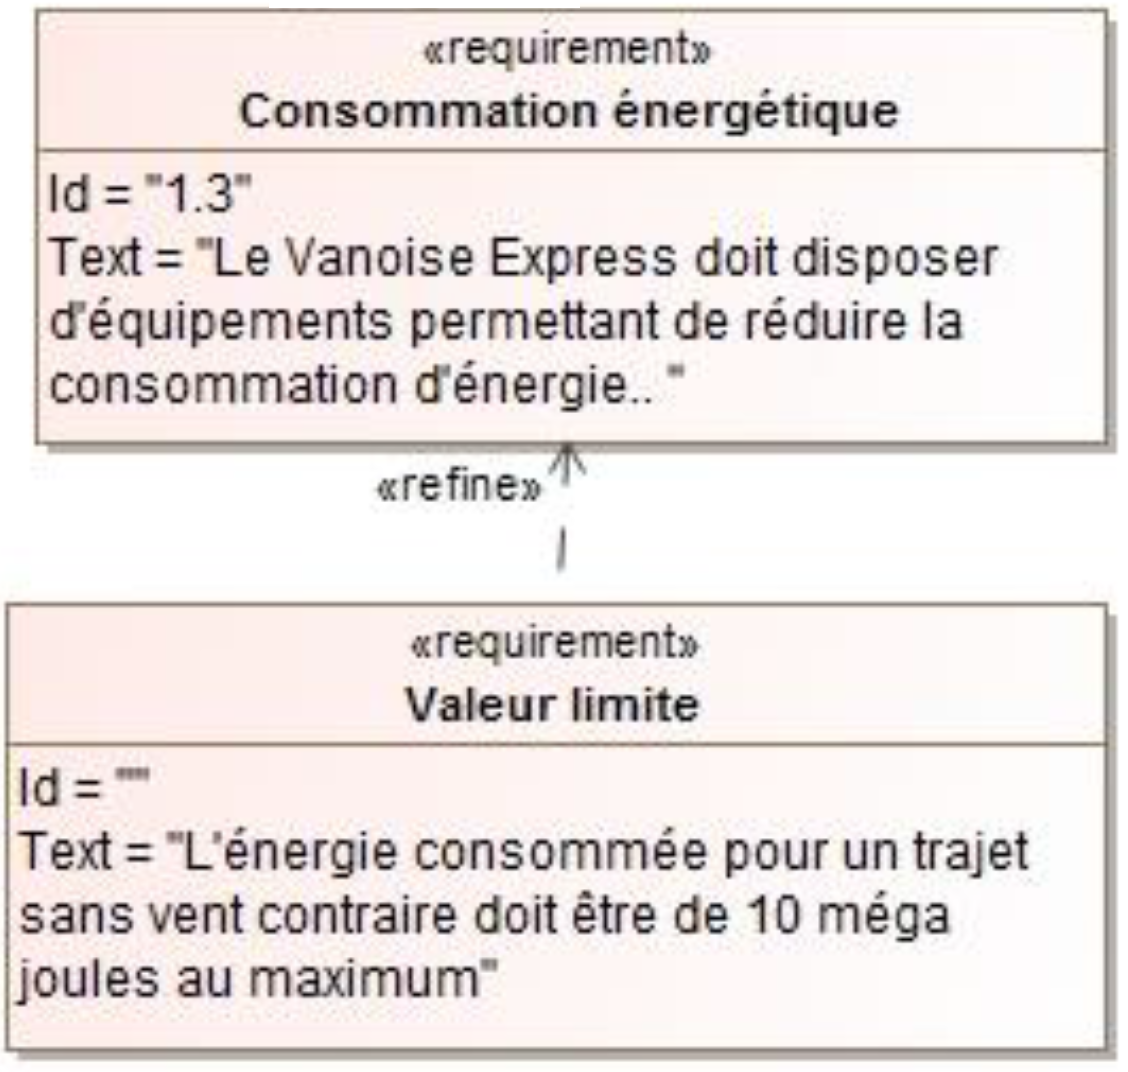
\includegraphics[width=0.3\linewidth]{img/fig16}
\caption{Exigence 1.3}
\label{fig16}
\end{figure}

\section{Vérification des critères \og Durée trajet \fg  et \og Distance d'arrêt \fg (15 min)}

Les exigences \og 1.2.1.1 \fg et \og 1.4 \fg vont être vérifiées dans cette partie.

Les moteurs du téléphérique sont asservis en vitesse. La consigne est décrite sur la figure ci-dessous. L'immobilisation en gare est assurée par une consigne de vitesse nulle et par le frein à patin de service (frein à desserrage hydraulique).

\begin{figure}[!h]
\centering
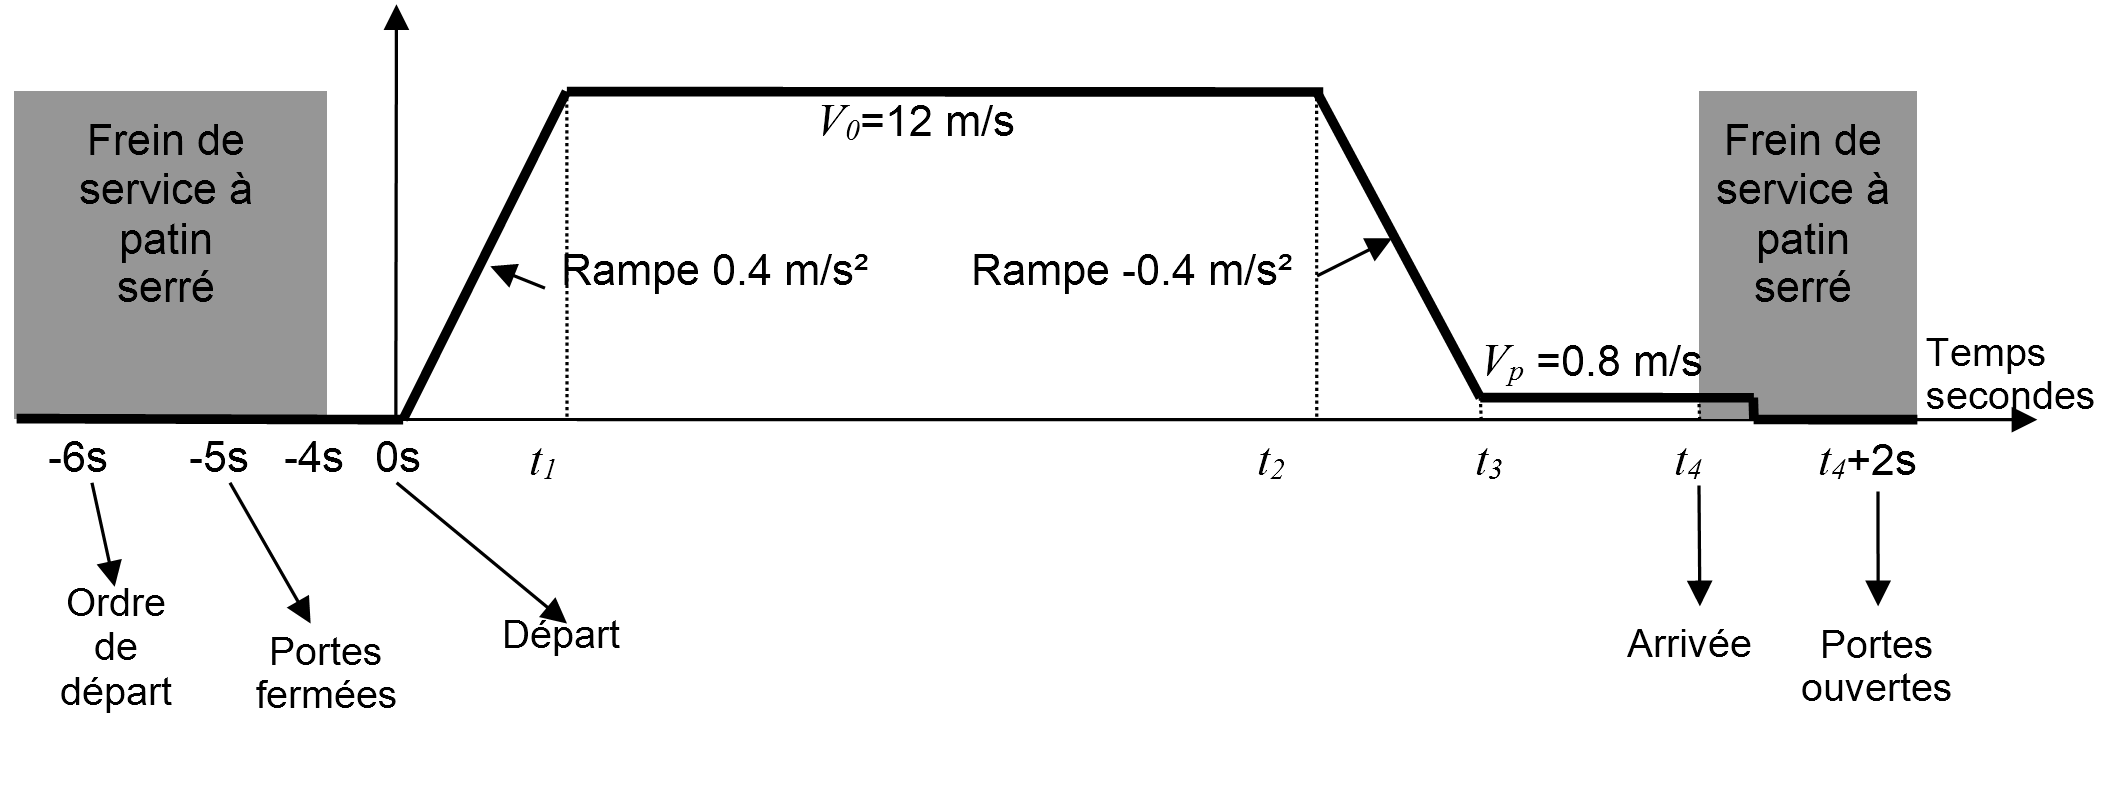
\includegraphics[width=0.8\linewidth]{img/fig17}
\caption{Consigne de vitesse pour un trajet au départ des Arcs à destination de La Plagne}
\label{fig17}
\end{figure}

Données :
\begin{itemize}
 \item La distance totale à parcourir est $d_t=1830$ mètres,
 \item Entre l'ordre de départ et le départ, 6 secondes s'écoulent,
 \item Entre l'arrivée et l'ouverture des portes, 2 secondes s'écoulent,
 \item Le départ a lieu à l'instant $t=0s$, l'arrivée à l'instant $t_4$,
 \item Les instants $t_1$, $t_2$ et $t_3$ marquent les changements de consigne de vitesse.
\end{itemize}

\paragraph{Question 1 :} Pour cette question, on demande des résultats numériques avec 4 chiffres significatifs à exprimer en secondes ou mètres (unités SI).

\begin{enumerate}
 \item Calculez numériquement $t_4-t_3$ pour respecter le critère de l'exigence : « Distance à parcourir en petite vitesse avant l'arrivée en gare »,
 \item Calculez numériquement $t_1$. En déduire numériquement la distance parcourue $d_a$ dans la phase d'accélération à $0.4m.s^{-2}$,
 \item Calculez numériquement $t_3-t_2$. En déduire numériquement la distance parcourue $d_d$ dans la phase de décélération à $-0.4m.s^{-2}$,
 \item Calculez numériquement $t_2-t_1$,
 \item Calculez numériquement la durée totale $t_t$ de l'ordre de départ jusqu'à l'ouverture des portes. Vérifiez le critère: « Durée d'un trajet (de l'ordre de départ jusqu'à l'ouverture des portes).
\end{enumerate}

\section{Vérification des critères de la fonction \og Freiner la cabine mécaniquement \fg (40 min)}

Dans cette partie, l'exigence \og 1.1.1.2.1 \fg sera vérifiée.

On peut voir sur l'annexe 1 qu'il existe 4 freins à patin identiques, 2 pour le freinage de service et 2 pour le freinage de secours (en cas de défaillance du précédent).

On appelle frein à patin l'unité décrite sur le schéma et sur le plan en coupe ci-dessous.

Pour des raisons de sécurité, les freins à patin de service seuls et sans énergie extérieure doivent être suffisants pour maintenir le téléphérique à l'arrêt quand il est en gare.

Chaque frein à patin possède un piston mobile qui se déplace dans un cylindre fixe. Le patin vient frotter sur la poulie motrice, produisant un moment de freinage.

C'est un frein de sécurité car sa force de freinage est obtenue sans énergie, par un ressort constitué de 18 rondelles élastiques de type Belleville. Ainsi, en l'absence (ou en cas de défaillance) de la pression hydraulique, le frein est serré. L'huile arrive par l'orifice « Arrivée d'huile » et la pression hydraulique permet seulement de desserrer le frein.

\begin{figure}[!h]
\centering
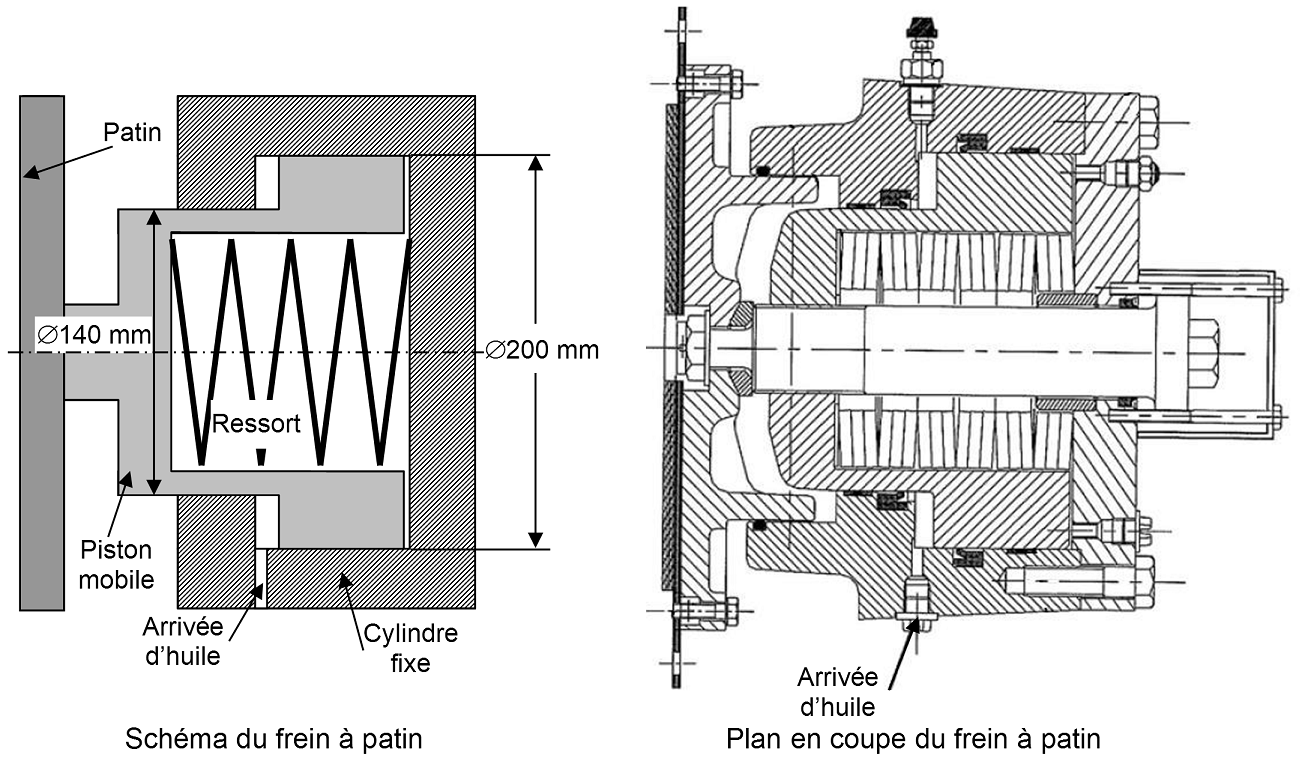
\includegraphics[width=0.68\linewidth]{img/fig18}
\caption{Frein à patin}
\label{fig18}
\end{figure}

Hypothèses et données :
\begin{itemize}
 \item On néglige l'effet du poids du câble tracteur (bien que très lourd, cette hypothèse est vraisemblable car le câble est porté par une trentaine de cavaliers),
 \item Seuls les 2 freins à patin de service sont actionnés,
 \item Tous les ressorts présents dans les freins à patin exercent la même action mécanique. On note $T_{ress\ mini}$ la plus petite tension du ressort qui permet l'équilibre de la cabine,
 \item Les moteurs électriques ne sont pas alimentés,
 \item La masse de la cabine est $M=29$ tonnes (chargement maximum). La masse du chariot est négligée,
 \item Le téléphérique est stationné en gare des Arcs. Le câble porteur est incliné de $\alpha=15\degree$ avec l'horizontale.,
 \item Les liaisons sont sans frottement (sauf bien sûr les deux liaisons par adhérence étudiées ici),
 \item Le coefficient d'adhérence entre le patin et la poulie motrice est  =0.3,
 \item La masse du contrepoids en gare de La Plagne est Mc=35 tonnes,
 \item Le diamètre des poulies de déviation est d=3.8 mètres,
 \item Le diamètre de la poulie motrice est D=4 mètres,
 \item On donne $g=9,81 m.s^{-2}$ (accélération de la pesanteur).
\end{itemize}

\paragraph{Question 2:}

\begin{wrapfigure}{r}{50mm}
	\vspace{-20pt}
	\centering 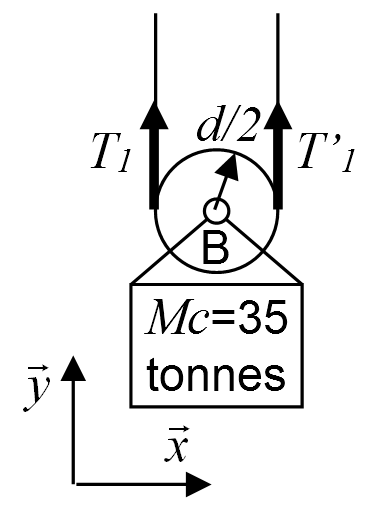
\includegraphics[width=0.7\linewidth]{img/fig19}
	\label{fig19}
\end{wrapfigure}

\begin{enumerate}
 \item On note $T_1$ et $T'_1$ les tensions dans les brins du câble tracteur, au niveau de la poulie de déviation soutenant le contrepoids. Montrez que $T_1=T'_1$. Précisez le solide isolé, et le principe ou théorème utilisé,
\item Montrez que $T_1=\frac{Mc.g}{2}$. Précisez le solide isolé, et le principe ou théorème utilisé.
\end{enumerate}

~\

\paragraph{Question 3:}

\begin{wrapfigure}{r}{70mm}
	\vspace{-20pt}
	\centering 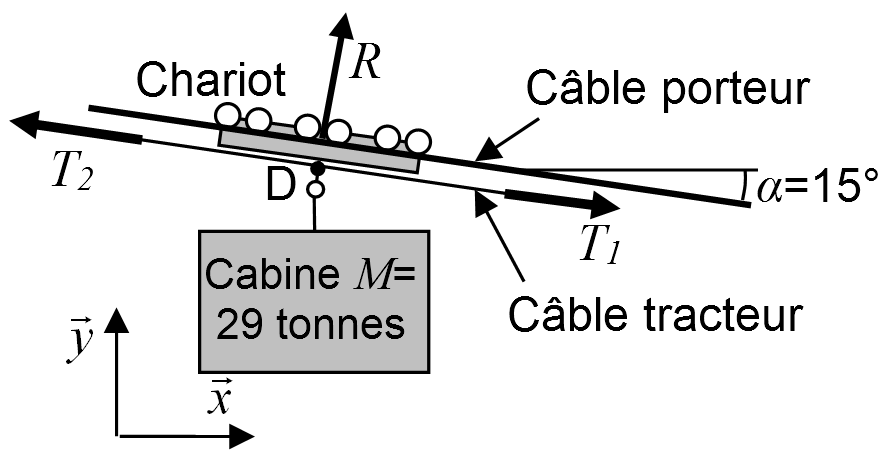
\includegraphics[width=0.8\linewidth]{img/fig20}
	\label{fig20}
\end{wrapfigure}

L'action mécanique du câble sur le chariot est modélisée comme un glisseur, de direction perpendiculaire au câble et de norme R.
Calculez numériquement la tension $T_2$ du câble tracteur côté Les Arcs. Précisez le ou les solides isolés, et le principe ou théorème utilisé.

~\ \\

\paragraph{Question 4:}

\begin{wrapfigure}{r}{60mm}
	\vspace{-20pt}
	\centering 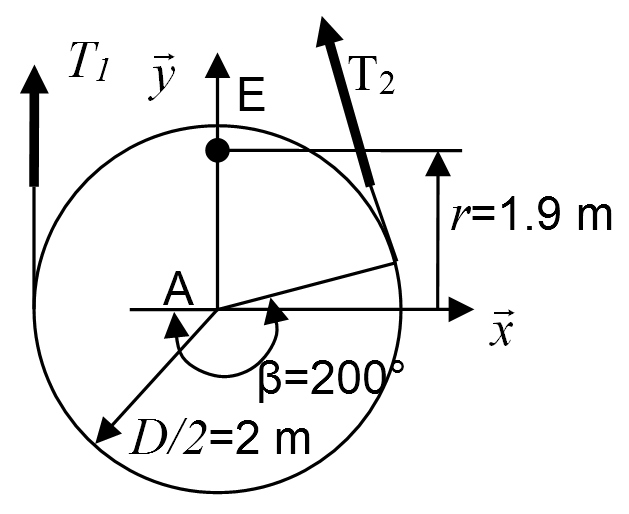
\includegraphics[width=0.8\linewidth]{img/fig21}
	\label{fig21}
\end{wrapfigure}

Les freins à patin de service agissent des deux côtés de la poulie en E et E' sur un rayon r=1.9 m. L'action de chaque frein de service sur la poulie sera modélisée par un glisseur. La tension des ressorts est $T_{ress\ mini}$. On se place à la limite du glissement.
\begin{enumerate}
 \item Isolez la poulie motrice. En explicitant le principe ou théorème utilisé, donnez l'expression de la tension $T_{ress\ mini}$ de chaque ressort en fonction de $T_1$, $T_2$, $r$, $D$ et $tan \varphi$.
 \item Calculez numériquement $T_{ress\ mini}$.
\end{enumerate}

~\

\begin{wrapfigure}{r}{50mm}
	\vspace{-20pt}
	\centering 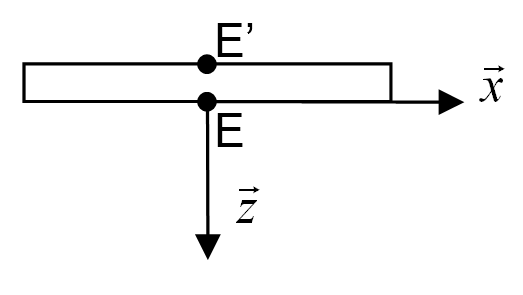
\includegraphics[width=0.8\linewidth]{img/fig22}
	\label{fig22}
\end{wrapfigure}
 
Pour des raisons de sécurité, on admettra que la tension $T_{ress\ mini}$ doit être multipliée au moins par un coefficient s=2 appelé coefficient de sécurité. On note $T_{ress\ secu}=2.T_{ress\ mini}$,
Vérifiez si le niveau du critère \og Tension du ressort des freins à patin pour immobiliser le téléphérique en gare, sans énergie extérieure \fg est suffisant.

Dans la suite, l'exigence \og 1.1.1.2.2 \fg sera vérifiée.

Le desserrage du frein à patin se fait par injection d'huile sous pression par l'orifice « Arrivée d'huile », visible sur le schéma du frein à patin \ref{fig18}.

Hypothèses et données :
\begin{itemize}
 \item Chaque ressort du frein à patin délivre une tension $T_{ress}=280kN$, supposée constante car les déplacements sont faibles,
 \item Les données dimensionnelles sont indiquées sur le schéma du frein à patin \ref{fig18},
 \item Les liaisons sont sans frottement.
\end{itemize}

\paragraph{Question 5 :}

\begin{itemize}
 \item Calculez numériquement la pression minimum $P_{min}$ que doit exercer l'huile sur le piston mobile pour comprimer le ressort,
 \item Vérifiez si le niveau du critère \og Pression de desserrage des freins à patin \fg est suffisant.
\end{itemize}

Dans la suite, l'exigence \og 1.1.1.2.3 \fg sera vérifiée.

Pour s'assurer que la cabine est bien à l'arrêt lorsque le frein à patin de service est serré, il faut encore vérifier que le câble ne peut pas glisser sur la poulie motrice. Nous allons donc calculer le coefficient d'adhérence $\nu_{mini}$ juste nécessaire pour assurer l'adhérence du câble sur la poulie motrice. On se place à la limite du glissement.

\begin{wrapfigure}{r}{50mm}
	\vspace{-20pt}
	\centering 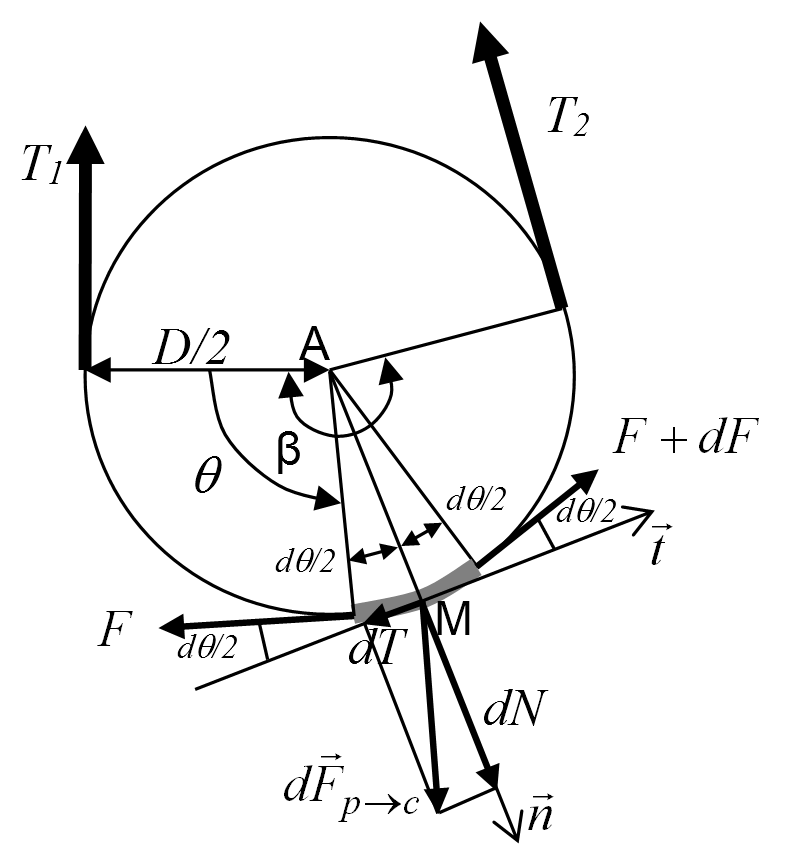
\includegraphics[width=0.8\linewidth]{img/fig23}
	\label{fig23}
\end{wrapfigure}

On isole un bout de câble de longueur $\frac{D}{2}.d\theta$. Il est soumis à trois forces extérieures : les tensions $F$ et $F+dF$, et l'action $d\overrightarrow{F_{p\rightarrow c}}$  de la poulie sur le câble.

Données et notations :
\begin{itemize}
 \item On donne $\beta=200\degree$ l'angle d'enroulement du câble, 
 \item On note $dN$, la composante normale de $d\overrightarrow{F_{p\rightarrow c}}$,
 \item On note $dT$, la composante tangentielle de $d\overrightarrow{F_{p\rightarrow c}}$,
 \item On note $\nu_{mini}$ le coefficient d'adhérence juste nécessaire pour assurer l'adhérence du câble sur la poulie motrice,
 \item Le câble enroulé sur la poulie est soumis à ses deux extrémités aux tensions $T_1$ et $T_2$ vues précédemment.
\end{itemize}


\paragraph{Question 6 :}
	
\begin{enumerate}
 \item Ecrire l'équation du théorème de la résultante statique appliqué au bout de câble isolé, linéarisée à l'ordre 1 en projection sur $\overrightarrow{n}$,
 \item Ecrire l'équation du théorème de la résultante statique appliqué au bout de câble isolé, linéarisée à l'ordre 1 en projection sur $\overrightarrow{t}$,
 \item En déduire une équation différentielle liant $F$, $dF$, $d\theta$ et $\nu_{mini}$.
\end{enumerate}

\paragraph{Question 7 :} Après avoir intégré cette équation différentielle, en déduire l'expression littérale de $\nu_{mini}$ en fonction du rapport $\frac{T_2}{T_1}$ et de $\beta$.

\paragraph{Question 8 :} Indépendamment de ce qui a été fait précédemment, on donne $\frac{T_2}{T_1}=1.5$.

\begin{enumerate}
 \item Calculez numériquement $\nu_{mini}$,
 \item Pour des raisons de sécurité, on ne peut pas être à la limite du glissement. On admettra que $\nu_{mini}$ doit être multiplié au moins par un coefficient $s=2$ appelé coefficient de sécurité. On note $\nu_{mini\ secu}=2.\nu_{mini}$. Vérifiez si le niveau du critère \og Coefficient d'adhérence entre la poulie motrice et le câble tracteur pour immobiliser le téléphérique en gare \fg est suffisant.
\end{enumerate}

\section{Vérification des critères \og Vitesse maximum de la cabine \fg et \og Durée d'arrêt par freinage mécanique de la cabine \fg (30 min)}

\begin{wrapfigure}{r}{60mm}
	\vspace{-10pt}
	\centering 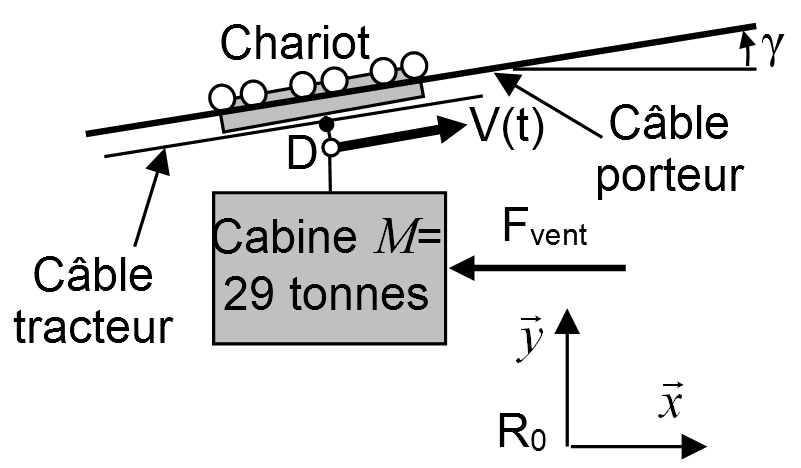
\includegraphics[width=0.8\linewidth]{img/fig24}
	\label{fig24}
\end{wrapfigure}

Hypothèses et données :
\begin{itemize}
 \item Soir $R_0$, un repère galiléen lié à la terre,
 \item On donne $g=9.81 m.s^{-2}$, accélération de la pesanteur,
 \item Soit (E), le système matériel constitué de tous les solides en mouvement et du câble tracteur,
 \item On suppose que la cabine de masse M=29 tonnes se déplace en translation à la vitesse $V(t)$, sur le câble incliné de $\gamma$ par rapport à l'horizontale (voir figure ci-contre),
\end{itemize}

\begin{itemize}
 \item La poulie motrice a pour moment d'inertie par rapport à son axe $J_{pm}=17 000 kg.m^2$. Son diamètre est $D=4m$. Sa vitesse de rotation est notée $\omega(t)$,
 \item Chacune des 5 poulies de déviation a pour moment d'inertie $J_d=10 500 kg.m^2$ et pour diamètre $d=3.8m$,
 \item La masse totale du câble tracteur est m=29 tonnes. On suppose qu'il se déplace en translation à la vitesse $V(t)$. On néglige la puissance de la pesanteur sur le câble tracteur dans son mouvement par rapport à $R_0$,
 \item On néglige la masse du chariot et de ses poulies de guidage,
 \item La câble tracteur est guidé par 50 petites poulies de guidage dont les caractéristiques sont : moment d'inertie $J_g=2 kg.m^2$, diamètre $d_g=0.5m$. Trente deux de ces poulies sont montées sur des cavaliers accrochés aux câbles porteurs (voir annexe 1), les autres guident le câble en gare,
 \item Chaque moteur délivre la même puissance et a pour puissance maximum $P_{m,maxi}=530kW$. Chaque moteur a pour moment d'inertie $J_m=11.2kg.m^2$,
 \item On note $\omega_m(t)$ la vitesse de rotation d'un moteur,
 \item On néglige les inerties des réducteurs de rapport $k=1/20$ et de tous les solides non cités dans les hypothèses. La définition du rapport $k$ est donnée annexe 1,
 \item On suppose que toutes les liaisons pivot des solides du système matériel E avec le milieu extérieur sont sans frottement.
\end{itemize}

On rappelle que la puissance mécanique s'écrit $P_m=\left\{\begin{array}{c}\overrightarrow{R} \\ \overrightarrow{M}\end{array}\right\}\otimes\left\{\begin{array}{c}\overrightarrow{\Omega} \\ \overrightarrow{V}\end{array}\right\}=\overrightarrow{\Omega}.\overrightarrow{M}+\overrightarrow{V}.\overrightarrow{R}$.

Cette partie consiste à vérifier l'exigence \og 1.1.2.1 \fg.

Lorsque la cabine approche de la gare de La Plagne, elle doit gravir une pente de $\gamma=15\degree$. Nous allons calculer la puissance $P_m$ par moteur qui permet d'atteindre et donc de respecter le niveau du critère ci dessus.

Hypothèses complémentaires pour le respect du critère ci-dessus :
\begin{itemize}
 \item Chacun des deux moteurs délivre la puissance $P_m$,
 \item La vitesse de la cabine est constante et égale à $V_0=12m.s^{-1}$,
 \item La cabine gravit une pente de $\gamma=15°$,
 \item L'action du vent est modélisée par une force horizontale, s'opposant au déplacement, d'intensité constante $F_{vent}=5 000 N$. Cette force est un maximum obtenu uniquement par vent défavorable.
 \item $f=6 N.m.s.rad^{-1}$ coefficient de frottement visqueux équivalent de toutes les forces internes de frottement ramené sur l'axe du moteur, ils génèrent une puissance intérieure $P_{int}=-f.\omega_m^2(t)$.
\end{itemize}

\paragraph{Question 9 :}

\begin{enumerate}
 \item Donnez l'expression de $P_{Ext}$, la somme des puissances extérieures au système matériel E dans son mouvement par rapport au référentiel $R_0$.
\end{enumerate}

\paragraph{Question 10 :} Donnez l'expression de la vitesse de rotation $\omega_m(t)$ d'un moteur en fonction de la vitesse $V(t)$ de la cabine, du rapport $k$ et du diamètre $D$ de la poulie motrice.

\paragraph{Question 11 :}

\begin{enumerate}
 \item D'après le théorème de l'énergie cinétique, on a $P_{int}+P_{ext}=0$. Donnez l'expression de la puissance $P_m$ délivrée par chaque moteur en fonction de $k$, $V_0$, $D$, $M$, $g$, $f$, $\gamma$ et $F_{Vent}$. 
 \item Faire l'application numérique de $P_m$. Les moteurs choisis ont une puissance maximum $P_{m,maxi}=530kW$. Permettent-ils de respecter le niveau du critère « Vitesse maximum de la cabine dans une pente à 15° avec un vent défavorable » ? 
\end{enumerate}	

\section{Vérification des critères \og Écart statique \fg et \og Écart de traînage \fg (1h10)}

Dans ce qui suit, on désire respecter l'exigence \og 1.1.2.2 \fg du cahier des charges.

En effet, afin de respecter les consignes de vitesse pour un trajet entre \og Les Arcs \fg et \og La Plagne \fg, il est nécessaire que l'asservissement de vitesse des moteurs à courant continu ait des qualités en précision, stabilité et rapidité.

\textbf{Modélisation des moteurs à courant continu}

\begin{wrapfigure}{r}{70mm}
	\vspace{-20pt}
	\centering 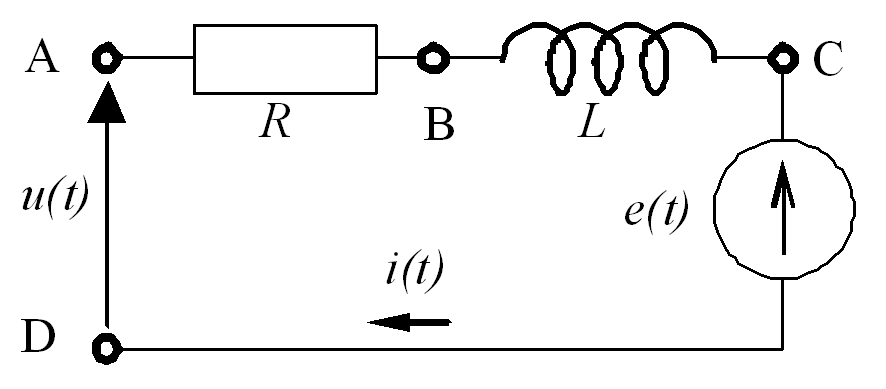
\includegraphics[width=0.8\linewidth]{img/fig25}
	\label{fig25}
\end{wrapfigure}

Notations :
\begin{itemize}
 \item On notera $F(p)$ la transformée de Laplace d'une fonction du temps $f(t)$,
 \item $u(t)$ Tension d'alimentation des moteurs,
 \item $i(t)$ Intensité traversant un moteur,
 \item $e(t)$ Force contre électromotrice d'un moteur,
 \item $\omega_m(t)$ Vitesse de rotation d'un moteur,
 \item $c_m(t)$ Couple d'un seul moteur,
 \item $c_r(t)$ Couple de perturbation engendré par le poids du téléphérique dans une pente et par l'action du vent, ramené sur l'axe des moteurs.
\end{itemize}

Hypothèses et données :
\begin{itemize}
 \item On suppose les conditions initiales nulles,
 \item Les deux moteurs sont et fonctionnent de manière parfaitement identique,
 \item $L=0.59 mH$: Inductance d'un moteur,
 \item $R=0.0386\Omega$: Résistance interne d'un moteur,
 \item $f=6 N.m.s.rad^{-1}$: Coefficient de frottement visqueux équivalent ramené sur l'axe des moteurs,
 \item $J=800kg.m^2$: Moment d'inertie total des pièces en rotation, ramené sur l'axe des moteurs,
 \item $c_m(t)=k_T.i(t)$ avec $k_T=5.67Nm.A^{-1}$ (constante de couple d'un moteur),
 \item $e(t)=k_E.\omega_m(t)$ avec $k_E=5.77 Vs.rad^{-1}$ (constante électrique d'un moteur),
 \item Équations de la dynamique établie dans la partie précédente : $2.c_m(t)-c_r(t)=J.\dot{\omega_m}(t)+f.\omega_m(t)$
\end{itemize}	 

\paragraph{Question 12 :} Le schéma bloc de la double motorisation étant fourni ci-après, déterminez les fonctions de transfert  $G_1(p)$, $G_2(p)$, $G_3(p)$ et $G_4(p)$ écrites dans le domaine de Laplace.

\begin{figure}[!h]
\centering
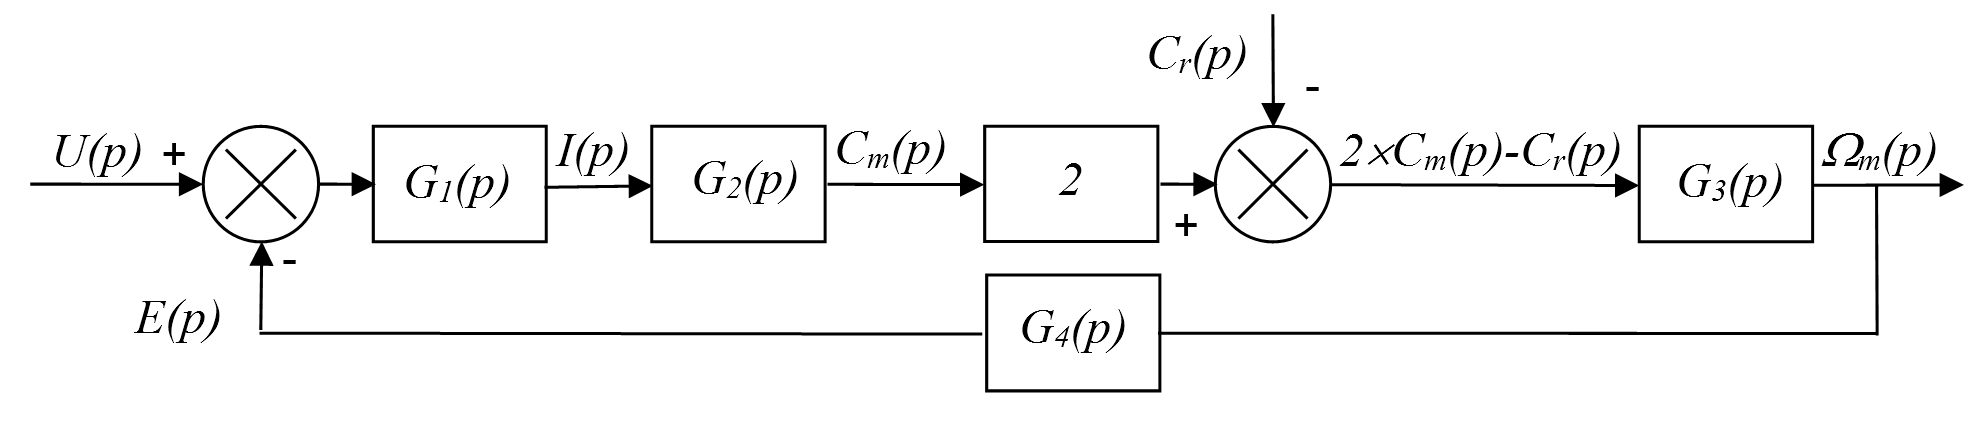
\includegraphics[width=0.8\linewidth]{img/fig26}
\label{fig26}
\end{figure}

\paragraph{Question 13 :} $\Omega_m(p)$ peut se mettre sous la forme :  $\Omega_m(p)=F_1(p).U(p)-F_2(p).C_r(p)$

Exprimez les fonctions $F_1(p)$ et $F_2(p)$ en fonction de $G_1(p)$, $G_2(p)$, $G_3(p)$ et $G_4(p)$	.

On donne en annexe 3 les résultats d'une simulation réalisée sur l'ensemble de la motorisation, constituée des deux moteurs à courant continu.

\begin{enumerate}
 \item La première courbe représente la réponse en vitesse à un échelon de tension $u(t)$ d'amplitude 100 V (le couple de perturbation $c_r(t)$ est nul).
 \item La seconde courbe représente la réponse en vitesse à un échelon de couple de perturbation $c_r(t)$ d'amplitude 1000 N.m (la tension $u(t)$ est nulle).
\end{enumerate}

\paragraph{Question 14 :} Choisissez et justifiez un modèle d'identification de ces fonctions (premier ordre, second ordre etc...). Déterminez numériquement les deux fonctions $F_1(p)$ et $F_2(p)$ par identification.

En faisant l'approximation que les deux fonctions $F_1(p)$ et $F_2(p)$ ont sensiblement le même dénominateur, le schéma bloc ci-dessus peut se mettre sous la forme suivante :

\begin{figure}[!h]
\centering
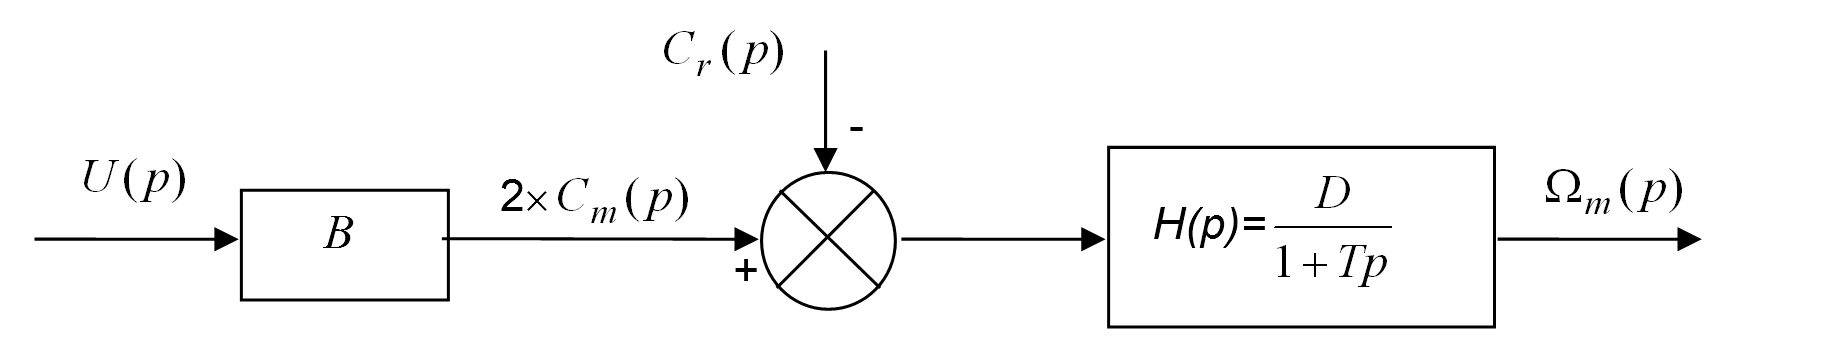
\includegraphics[width=0.8\linewidth]{img/fig27}
\label{fig27}
\end{figure}

\paragraph{Question 15 :} Donnez la valeur numérique des trois constantes $B$, $D$ et $T$.


La motorisation modélisée ci-dessus est insérée dans une boucle d'asservissement de vitesse.

\begin{figure}[!h]
\centering
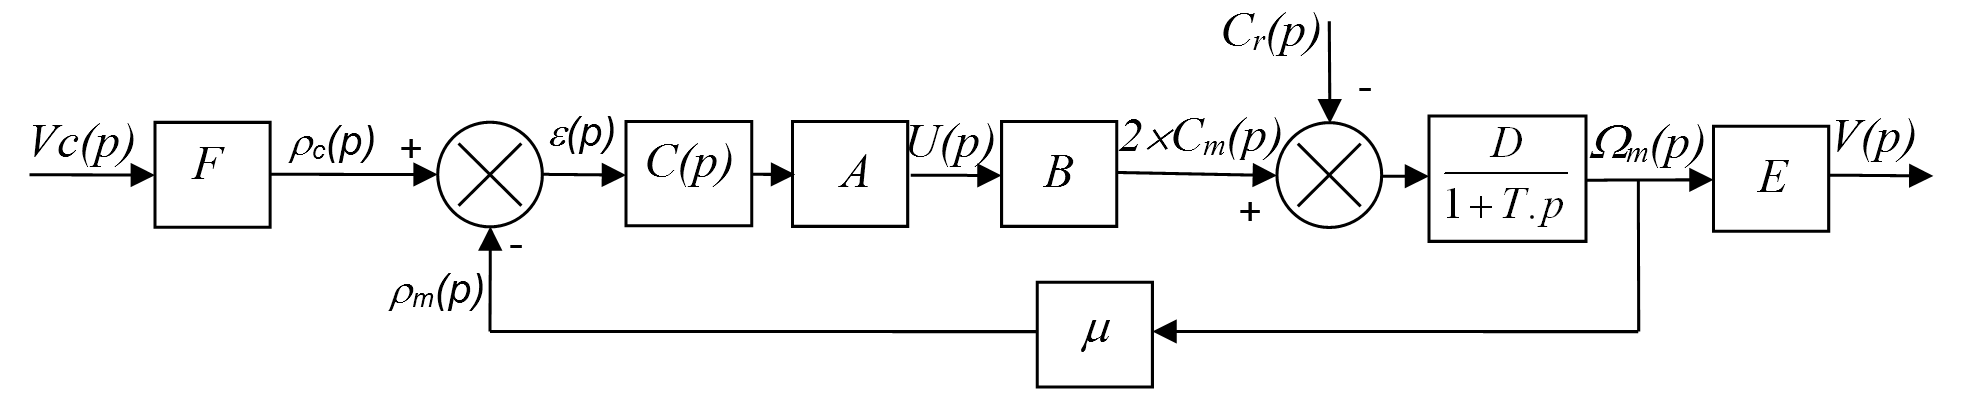
\includegraphics[width=0.8\linewidth]{img/fig28}
\label{fig28}
\end{figure}

\begin{itemize}
 \item La consigne de vitesse $v_c(t)$ est donnée en entrée. Elle est convertie en une tension $\rho_c(t)$ avec le gain \og F \fg,
 \item Une génératrice tachymétrique de gain $\mu=0.716 V.s.rad^{-1}$ transforme la vitesse de rotation $\omega_m(t)$ du moteur en une tension $\rho_m(t)$,
 \item Un correcteur de fonction de transfert $C(p)$ corrige la différence $\epsilon(t)=\rho_c(t)-\rho_m(t)$ et l'envoie à un amplificateur de gain $A$, qui alimente les deux moteurs électriques,
 \item La vitesse de rotation des moteurs $\omega_m(t)$ est transformée en vitesse du téléphérique $v(t)$ avec le gain \og E \fg.
\end{itemize}

\paragraph{Question 16 :}

\begin{enumerate}
 \item Déterminez l'expression du gain \og E \fg. Faire une application numérique,
 \item Déterminez l'expression du gain \og F \fg pour que $\epsilon(t)=0$ entraîne $v_c(t)=v(t)$. Faire une application numérique.
\end{enumerate}

Par transformation du schéma bloc, le système est mis en retour unitaire. On obtient le résultat ci-dessous :

\begin{figure}[!h]
\centering
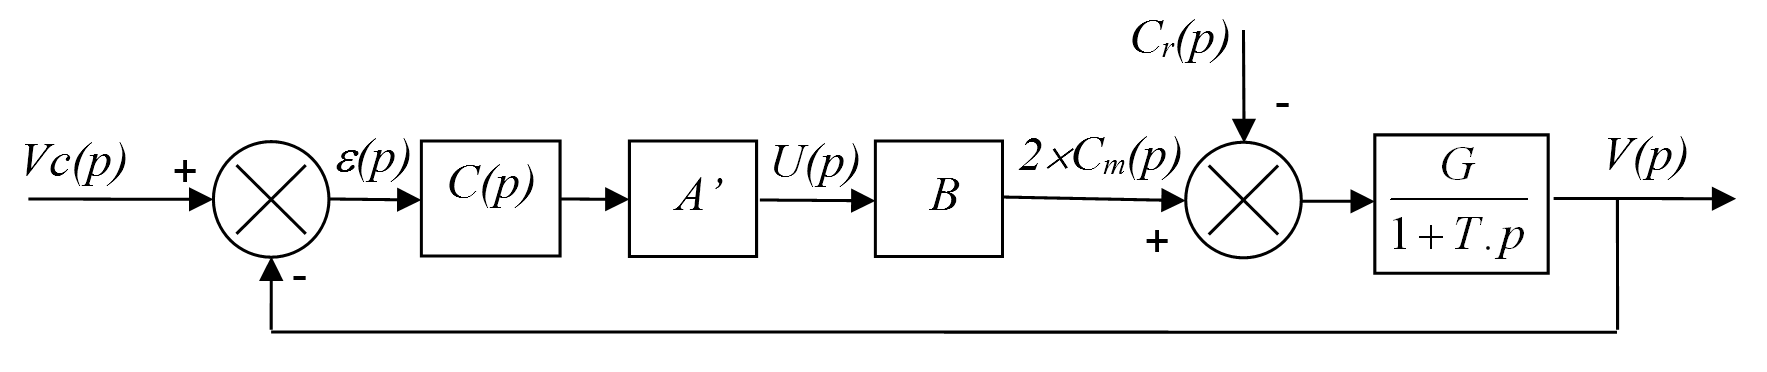
\includegraphics[width=0.8\linewidth]{img/fig29}
\label{fig29}
\end{figure}

Les coefficients $E$ et $F$ calculés précédemment sont intégrés dans les nouveaux coefficients $A'$ et $G$. Pour la suite, on continuera avec les valeurs suivantes : $A'.B=3.10^4s.N$, $G=6.10^{-5}m.(s.N.m)^{-1}$ et $T=0.47s$.

On se propose de tester successivement 3 correcteurs, et de retenir celui qui permet de respecter le cahier des charges.


\textbf{Utilisation d'un correcteur proportionnel :}   $C(p)=C_0=1$.

\paragraph{Question 17 :} Justifiez en quelques mots que le système est stable avec ce correcteur.

\paragraph{Question 18 :} On suppose $C_r(p)=0$. Calculez en fonction de $C_0$, $A'$, $B$, $G$, et $V_0$ l'expression de l'écart statique en suivi de consigne $\epsilon's$ engendré par une consigne en échelon d'amplitude $V_0=12m.s^{-1}$. Faire l'application numérique.

\paragraph{Question 19 :} On suppose $V_c(p)=0$.

\begin{enumerate}
 \item Calculez en fonction de $C_0$, $A'$, $B$, $G$, et $Cr_0$ l'expression de l'écart statique en régulation $\epsilon''s$ engendré par une perturbation échelon d'amplitude $Cr_0=-7270N.m$ qui modéliserait la descente des \og Arcs \fg. Faire l'application numérique,
 \item Faire également une application numérique si $Cr_0=+7460N.m$ pour la modélisation de la montée vers \og La Plagne \fg.
\end{enumerate}

\paragraph{Question 20 :} Donnez numériquement l'écart statique total $\epsilon=\epsilon's+\epsilon''s$  dans les deux cas suivants :
\begin{enumerate}
 \item Descente des \og Arcs \fg,
 \item Montée vers \og La Plagne \fg,
 \item Existe-t-il une valeur réaliste de $C_0$ pour laquelle le critère \og Écart statique en vitesse en présence d'une perturbation échelon \fg serait vérifié ? Justifiez.
\end{enumerate}
 
\textbf{Utilisation d'un correcteur intégral :} $C(p)=\frac{C_i}{p}$ Ce correcteur remplace le précédent.

\paragraph{Question 21 :} Donnez l'expression de la fonction de transfert en boucle ouverte du système, notée $FTBO(p)$. Faire l'application numérique pour $C_i=1$.

\paragraph{Question 22 :} Tracez le diagramme asymptotique de Bode de $FTBO(p)$. Tracez également l'allure des courbes.

\paragraph{Question 23 :}

\begin{enumerate}
 \item On suppose $C_r(p)=0$. Calculez numériquement l'écart statique en suivi de consigne $\epsilon's$ engendré par une consigne en échelon d'amplitude $V_0=12 m.s^{-1}$,
 \item On suppose $V_c(p)=0$. Calculez numériquement l'écart statique en régulation $\epsilon''s$ engendré par une perturbation échelon d'amplitude $Cr_0=-7270N.m$ qui modéliserait la descente des \og Arcs \fg,
 \item Donnez numériquement l'écart statique total $\epsilon_s=\epsilon's+\epsilon''s$. Le critère \og Écart statique en vitesse en présence d'une perturbations échelon \fg est-il vérifié ? Justifiez.
\end{enumerate}

\paragraph{Question 24 :} On suppose $C_r(p)=0$.

Calculez l'expression de l'écart de traînage $\epsilon_v$ engendré par une consigne en rampe unitaire. Existe-t-il une valeur de   réaliste qui permette de vérifier le critère \og Écart de traînage (ou écart dynamique) en vitesse en l'absence de perturbations \fg ? Justifiez.

\section{Vérification du critère \og Energie consommée \fg (10 min)}

Dans ce qui suit, on désire vérifier l'exigence \og 1.3 \fg.

Hypothèses : Dans un souci de simplification, la ligne entre \og Les Arcs \fg et \og La Plagne \fg a été modélisée de la manière suivante :

\begin{figure}[!h]
\centering
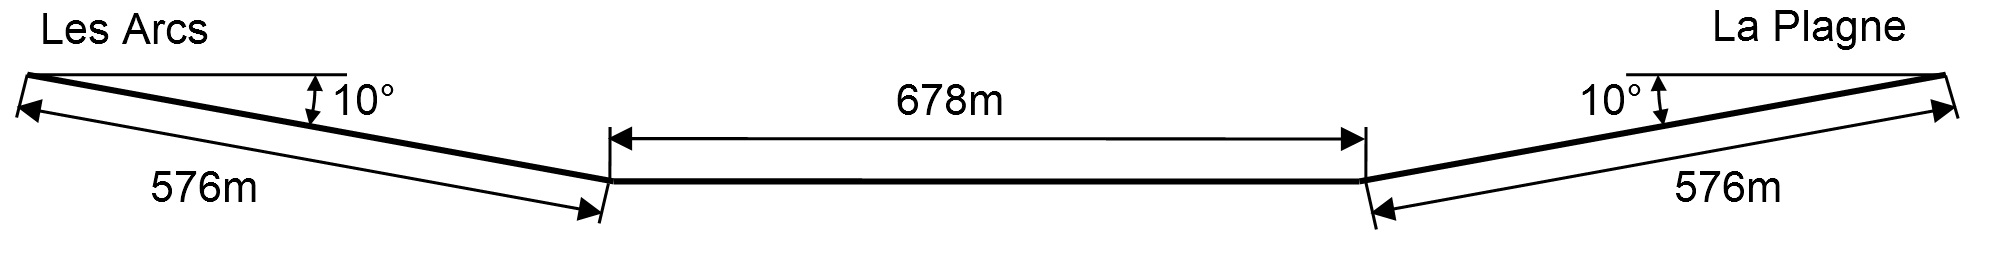
\includegraphics[width=0.8\linewidth]{img/fig30}
\label{fig30}
\end{figure}

En tenant compte de la résistance de l'air (sans vent) et de la pente, on a pu déterminer le couple de perturbation ramené sur l'axe des moteurs :

\begin{figure}[!h]
\centering
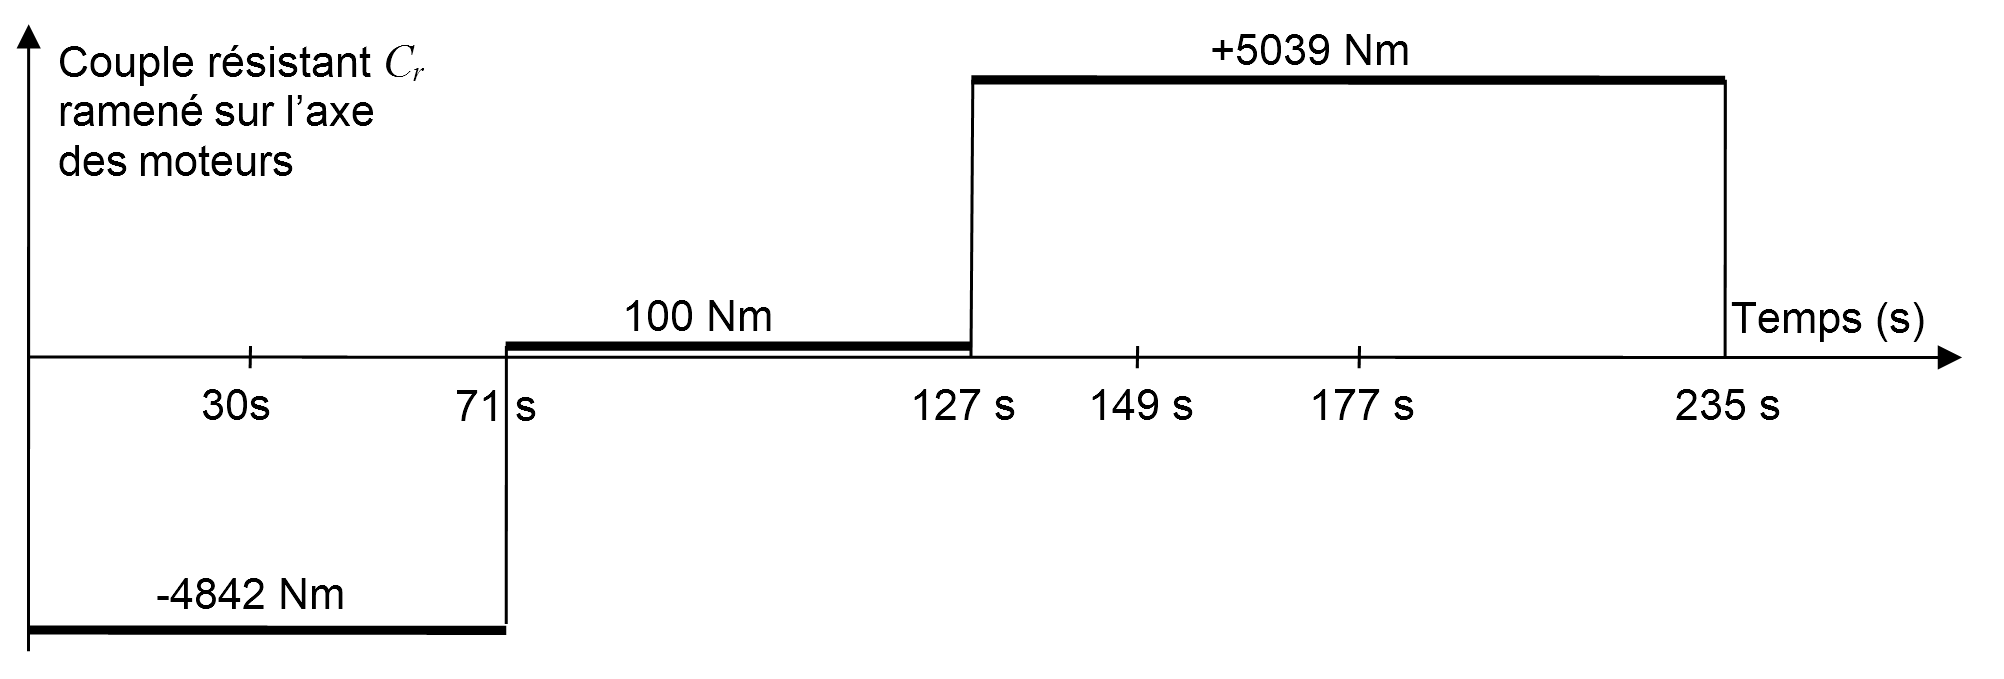
\includegraphics[width=0.8\linewidth]{img/fig31}
\label{fig31}
\end{figure}

Le modèle mis en place dans la partie précédente a permis de calculer la tension aux bornes d'un moteur, ainsi que l'intensité du courant électrique le traversant pendant les différentes phases du fonctionnement décrites dans la partie 3.

\begin{figure}[!h]
\centering
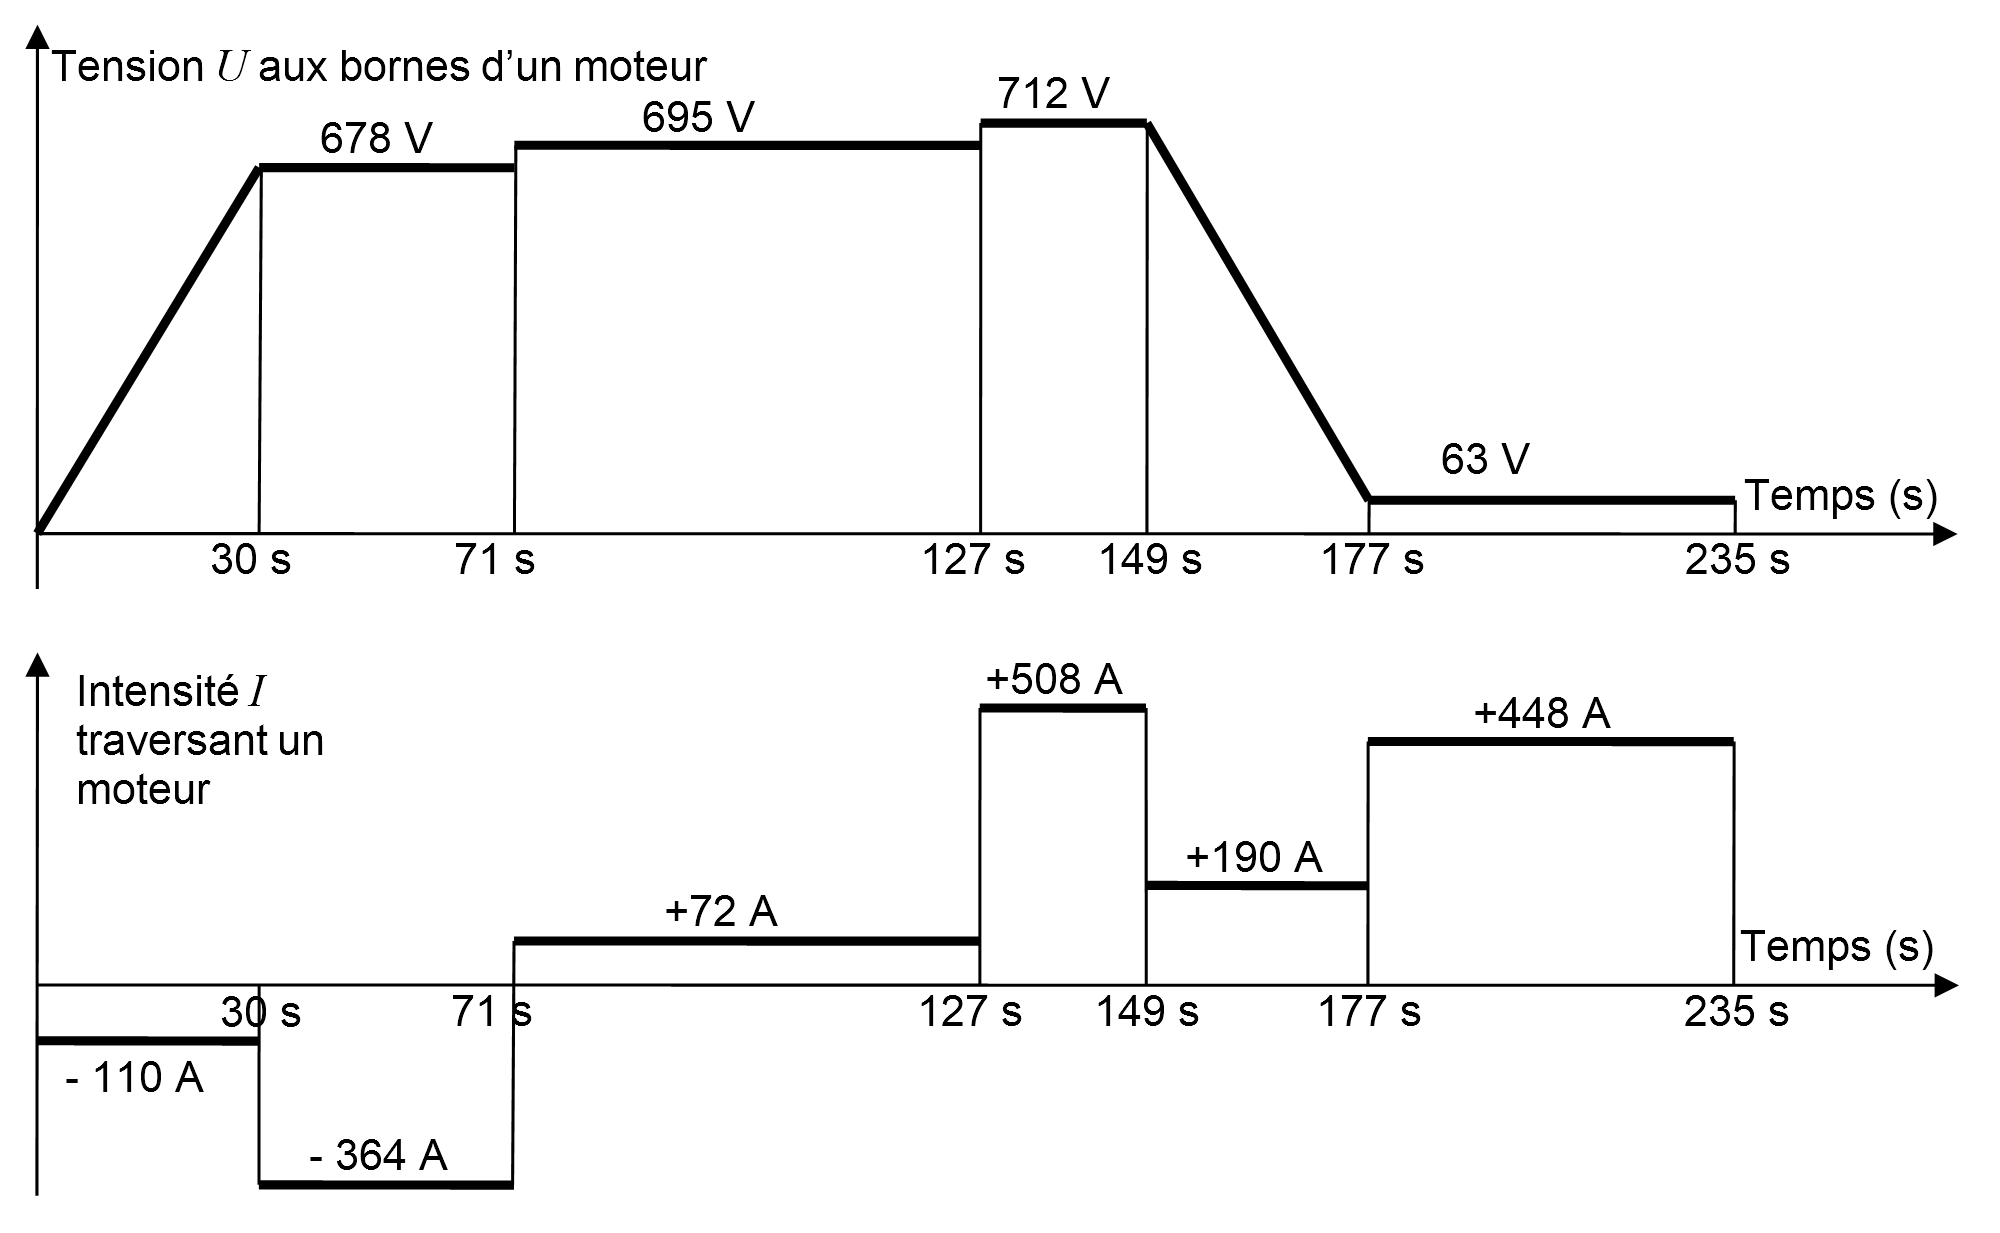
\includegraphics[width=0.8\linewidth]{img/fig32}
\label{fig32}
\end{figure}

Le Vanoise Express est équipé d'un système de récupération de l'énergie. Lorsque les moteurs doivent freiner le téléphérique, ils fonctionnent en génératrices, et l'énergie électrique qu'ils produisent est réinjectée dans le réseau EDF (avec un rendement que l'on supposera égal à 1).

D'après les courbes de tension et d'intensité, le trajet entre \og Les Arcs \fg et \og La Plagne \fg peut être découpé en 6 phases dont les instants sont indiqués en abscisse.

\paragraph{Question 25 :} On rappelle que les courbes de tension et d'intensité ne concernent qu'un seul moteur, et que les deux moteurs sont alimentés de la même manière.

\begin{enumerate}
 \item Pour chacune des 6 phases, calculez numériquement en Joules l'énergie $W_i$ (i variant de 1 à 6) produite ou consommée par le téléphérique, c'est-à-dire par l'ensemble des 2 moteurs,
 \item En déduire numériquement l'énergie $W$ consommée pour le trajet entre \og Les Arcs \fg et \og La Plagne \fg. Calculez en euros le coût d'un trajet sur une base de 12 centimes le kilowattheure (remarque : le kilowattheure est une unité de mesure d'énergie correspondant à l'énergie consommée par un appareil de 1 kW de puissance pendant une durée d'une heure). Le critère \og Énergie consommée pour un trajet sans vent contraire. \fg est-il vérifié ? Justifiez.
 \item Quelle énergie $W_{Max}$ aurait-on consommée sans le système de récupération ? Conclure sur l'intérêt de ce dispositif de récupération d'énergie.
\end{enumerate}

\section{Conception partielle de l'exigence : \og Assurer la sécurité des passagers \fg (20 min)}

En cas de panne mécanique dans la salle des machines, le téléphérique risque d'être bloqué à 380 mètres au dessus du sol. Avec cette différence d'altitude, une descente en rappel (à l'aide d'une corde) des 200 passagers n'est pas possible. Si le temps est mauvais, l'intervention d'un hélicoptère ne l'est pas non plus. Les deux cabines étant indépendantes, il serait possible de garer celle qui fonctionne encore à côté de celle qui est en panne, et de faire passer les passagers de l'une à l'autre. Les ingénieurs ont préféré imaginer des solutions plus confortables pour les passagers, qui permettent de les amener à destination, avec seulement quelques minutes de retard.

Dans ce qui suit, on désire concevoir une solution technique pour répondre à l'exigence \og 1.2.3.1 \fg.

En cas de panne des deux moteurs principaux, il est possible de les désaccoupler grâce aux deux accouplements débrayables situés de part et d'autre de la poulie motrice. Le moteur de secours (voir schéma et photo 4 ci-dessous, photo 5 en annexe 2) peut alors être mis en service.

\begin{figure}[!h]
\centering
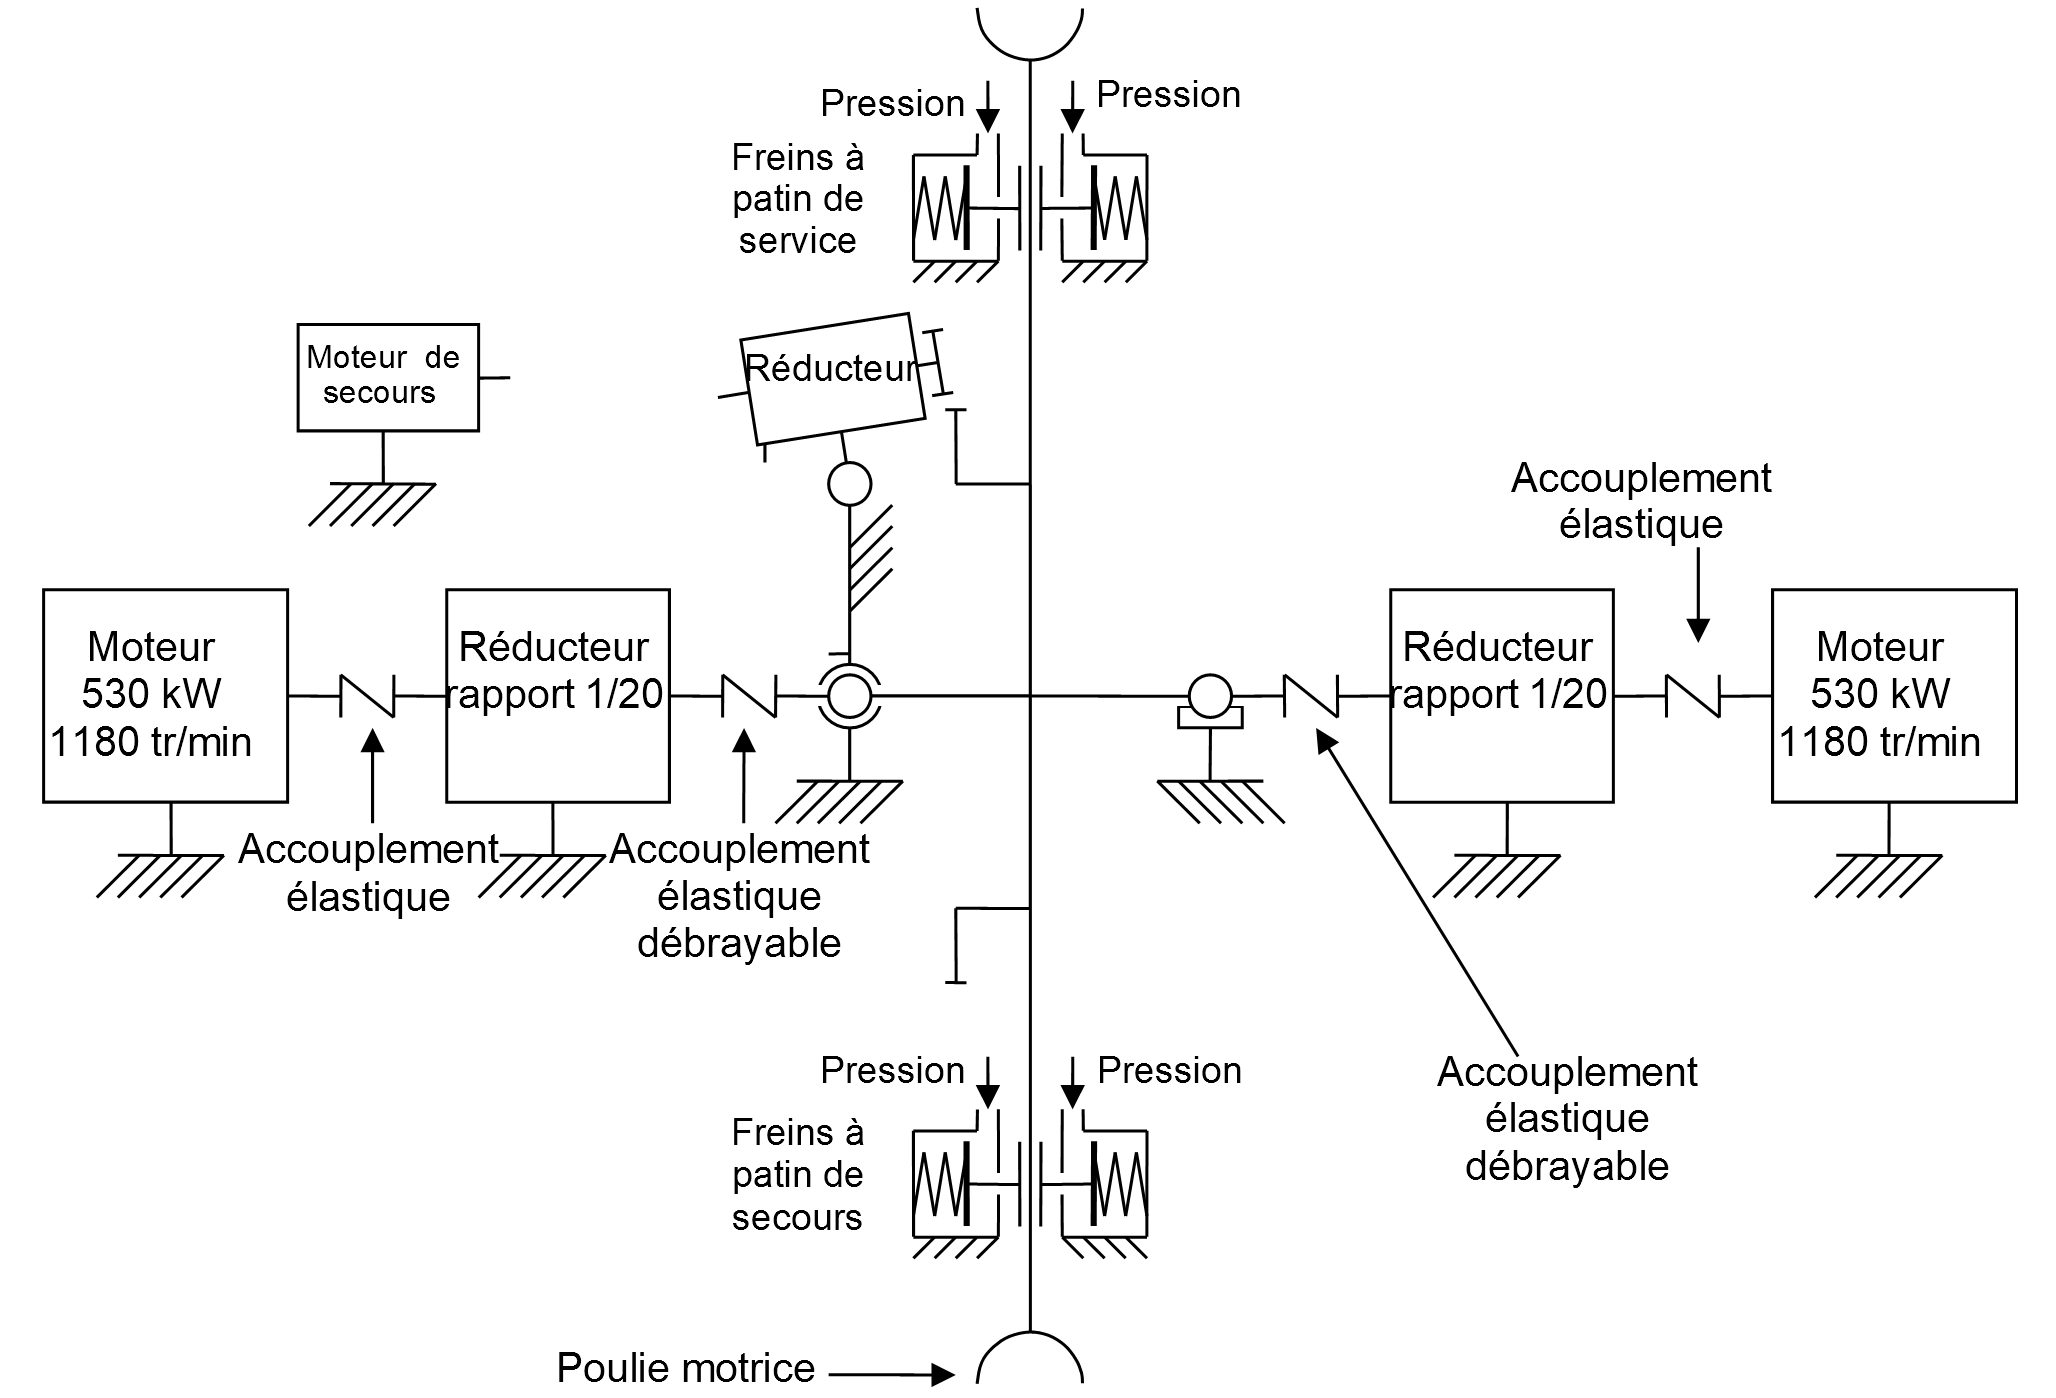
\includegraphics[width=0.9\linewidth]{img/fig33}
\label{fig33}
\end{figure}

\begin{figure}[!h]
\centering
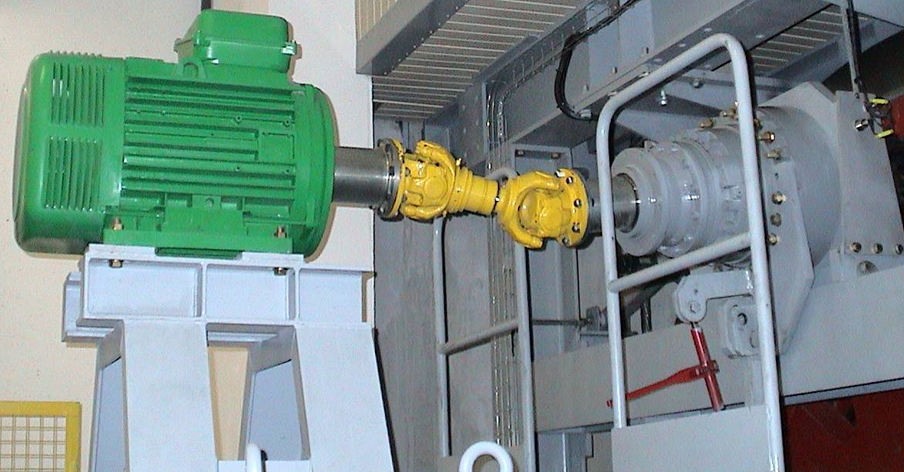
\includegraphics[width=0.8\linewidth]{img/fig34}
\caption{Moteur de secours et sa transmission (la zone à concevoir est masquée)}
\label{fig34}
\end{figure}

Sur le cahier réponse, on a représenté le moteur de secours et son réducteur de vitesse. A l'extrémité du réducteur, un pignon denté permet d'entraîner une roue dentée reliée à la poulie motrice. Le candidat remarquera que le réducteur est en liaison pivot avec le bâti. La rotation du réducteur permet la mise en service de ce dispositif de sécurité en amenant le pignon au contact de la roue dentée.

\paragraph{Question 26 :}
\begin{enumerate}
 \item Schématisez un dispositif de transformation de mouvement, permettant la mise en service du dispositif de sécurité en faisant pivoter le réducteur,
 \item Schématisez le dispositif de transmission de puissance à cardan, basé en particulier sur des liaisons rotule à doigt entre le moteur et le réducteur, permettant à l'arbre de transmission de s'articuler pour compenser des désalignements angulaires de 20° maximum (voir photo ci-dessus qui montre l'arbre de transmission en position désalignée).
\end{enumerate}

\newpage

\section{Conception de la liaison entre les poulies porte-câble et le bâti (40 min)}

L'objectif de cette partie est de concevoir la liaison pivot entre les poulies qui guident les câbles et le bâti.

\paragraph{Question 27:} Compléter le dessin d'ensemble du guidage en rotation de la poulie.

\begin{enumerate}
 \item Les deux roulements (roulements à une rangée de billes à contact radial) sont de même dimensions. Le diamètre de l'arbre utile en sortie est précisé sur le dessin,
 \item Les efforts proviennent principalement de la charge du câble,
 \item Une grande précision n'est pas ici fondamentale, mais une bonne résistance, une facilité de montage et d'entretien pour un graissage régulier sont recherchées,
 \item Une étanchéité par un joint à lèvre est nécessaire,
 \item Préciser les ajustements.
\end{enumerate}

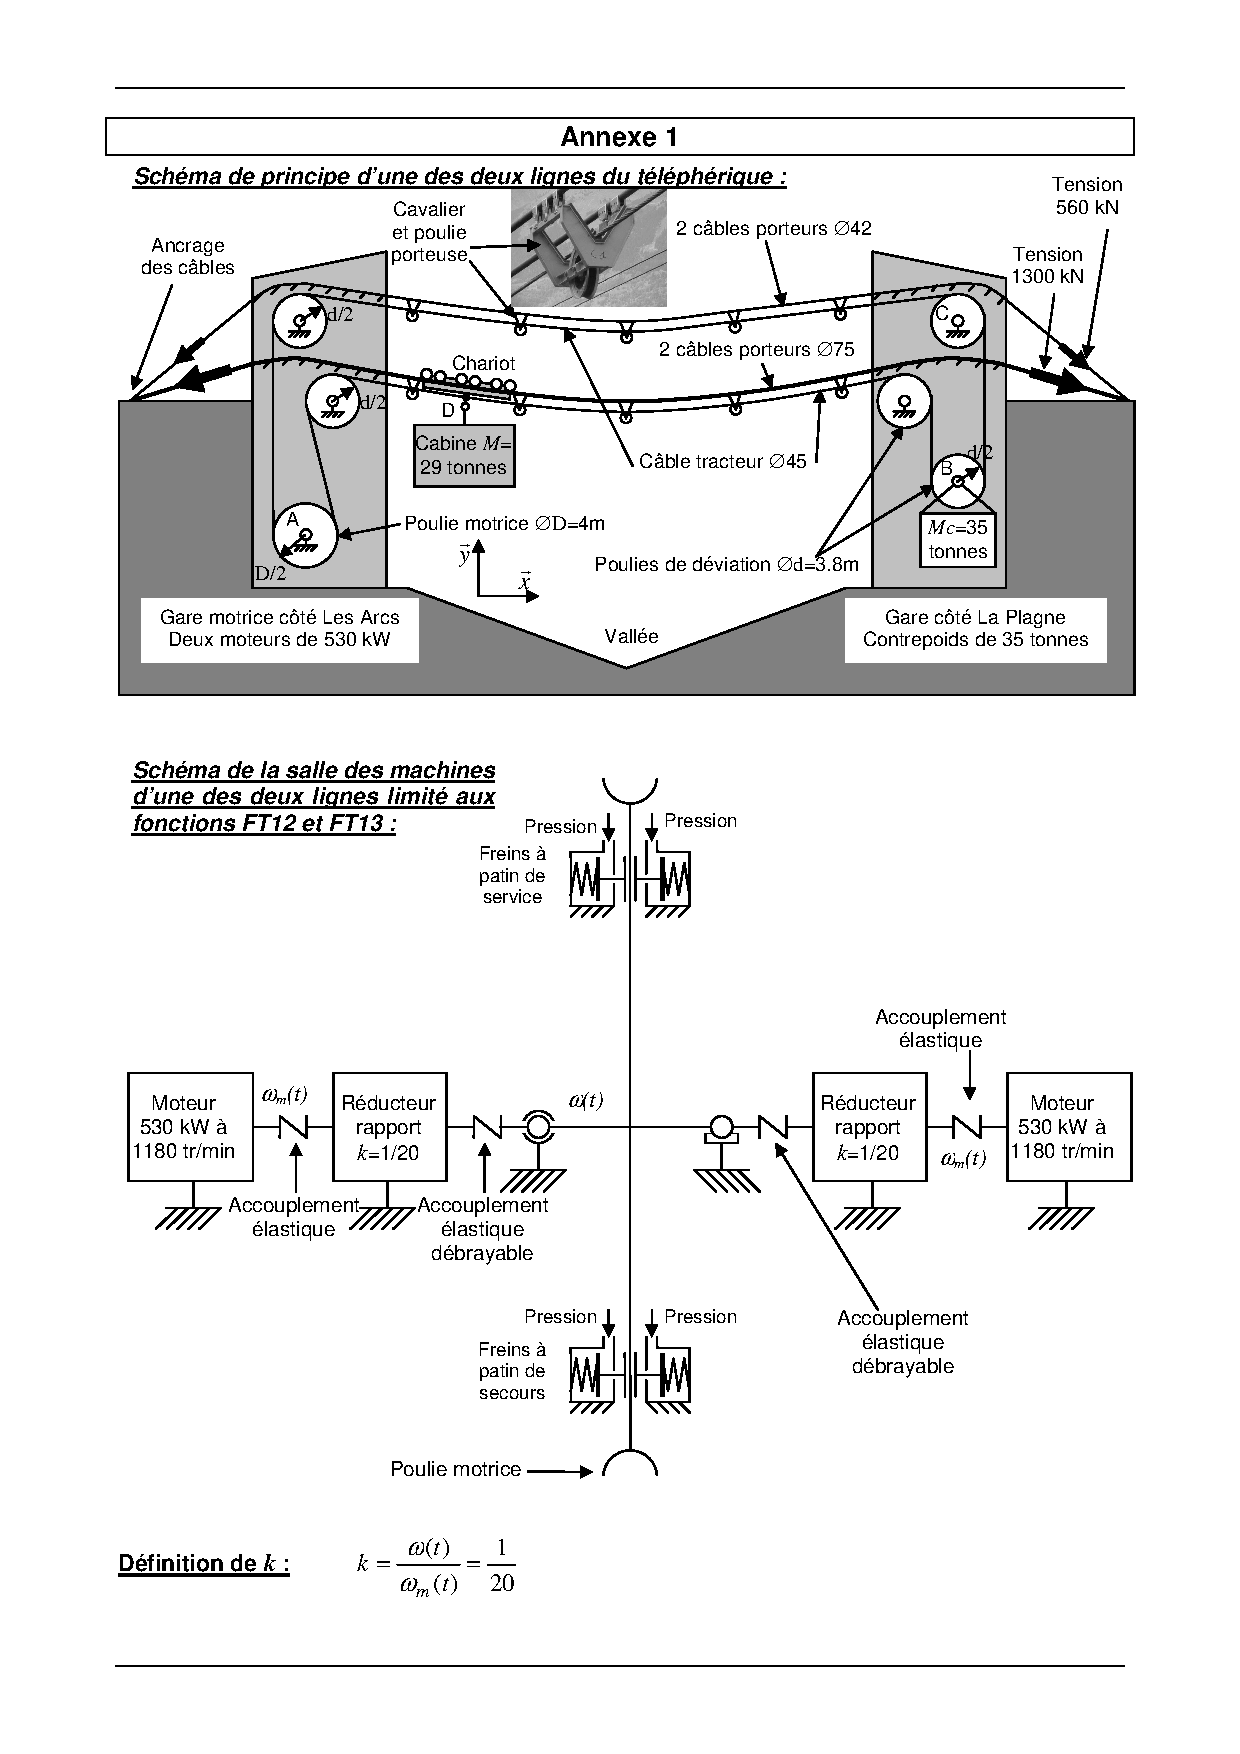
\includepdf[pages=1-4]{Annexes.pdf}

\paragraph{Éléments nécessaire à la conception}

\textbf{Joint à lèvre}

\begin{minipage}{0.3\linewidth}
 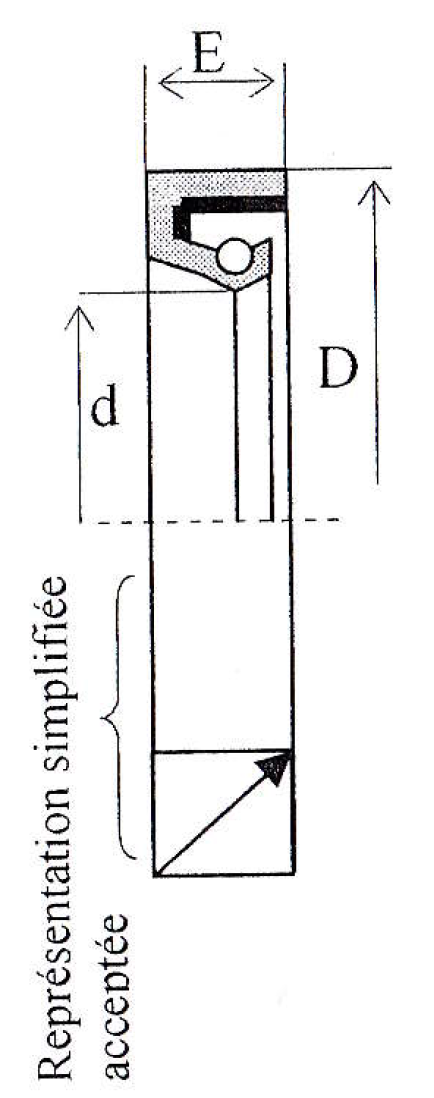
\includegraphics[width=0.6\linewidth]{img/dessin02}
\end{minipage}\hfill
\begin{minipage}{0.65\linewidth}
\begin{tabular}{|c|c|c|c|c|c|c|c|}
\hline
d & 18 & 20 & 22 & 25 & 28 & 30 & 32 \\
\hline
D & 35 & 38 & 40 & 42 & 45 & 48 & 50 \\
\hline
E & 8 & 8 & 8 & 8 & 8 & 8 & 8 \\
\hline
\end{tabular}
\end{minipage}

\textbf{Écrou à encoches}

\begin{minipage}{0.3\linewidth}
 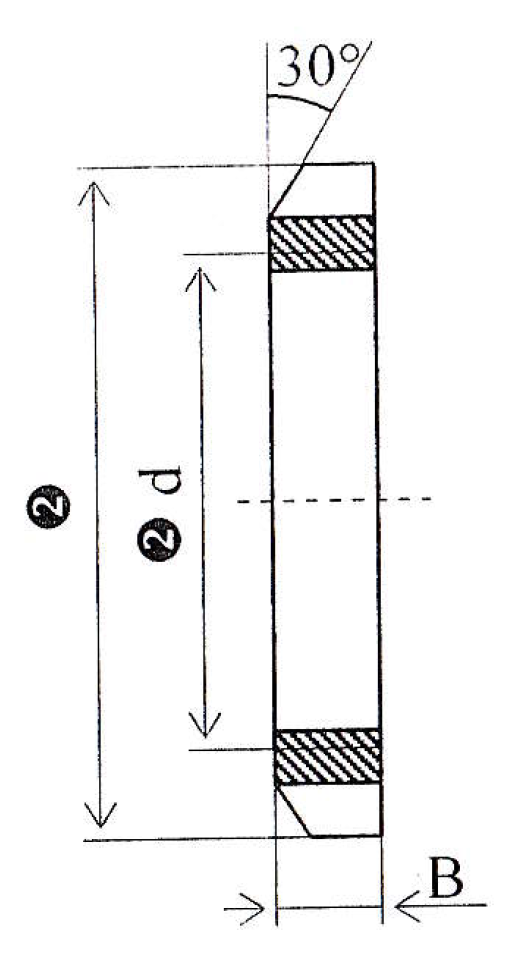
\includegraphics[width=0.6\linewidth]{img/dessin03}
\end{minipage}\hfill
\begin{minipage}{0.65\linewidth}
\begin{tabular}{|c|c|c|c|c|c|c|c|}
\hline
d & 15 & 17 & 20 & 25 & 28 & 30 & 32 \\
\hline
D & 25 & 28 & 32 & 38 & 42 & 45 & 48 \\
\hline
E & 5 & 5 & 6 & 7 & 7 & 7 & 8 \\
\hline
\end{tabular}
\end{minipage}

\cleardoublepage


\section{Document réponse}

\lhead{Nom:................. Prénom:...............}

\reponse{1}{25}

\reponse{2}{8}

\reponse{3}{6}

\reponse{4}{10}

\reponse{5}{7}

\reponse{6}{12}

\reponse{7}{5}

\reponse{8}{5}

\reponse{9}{10}

\reponse{10}{2}

\reponse{11}{6}

\reponse{12}{6}

\reponse{13}{6}

\reponse{14}{6}

\reponse{15}{4}

\reponse{16}{5}

\reponse{17}{2}

\reponse{18}{4}

\reponse{19}{6}

\reponse{20}{3}

\reponse{21}{3}

\reponse{22}{7}

\begin{center}
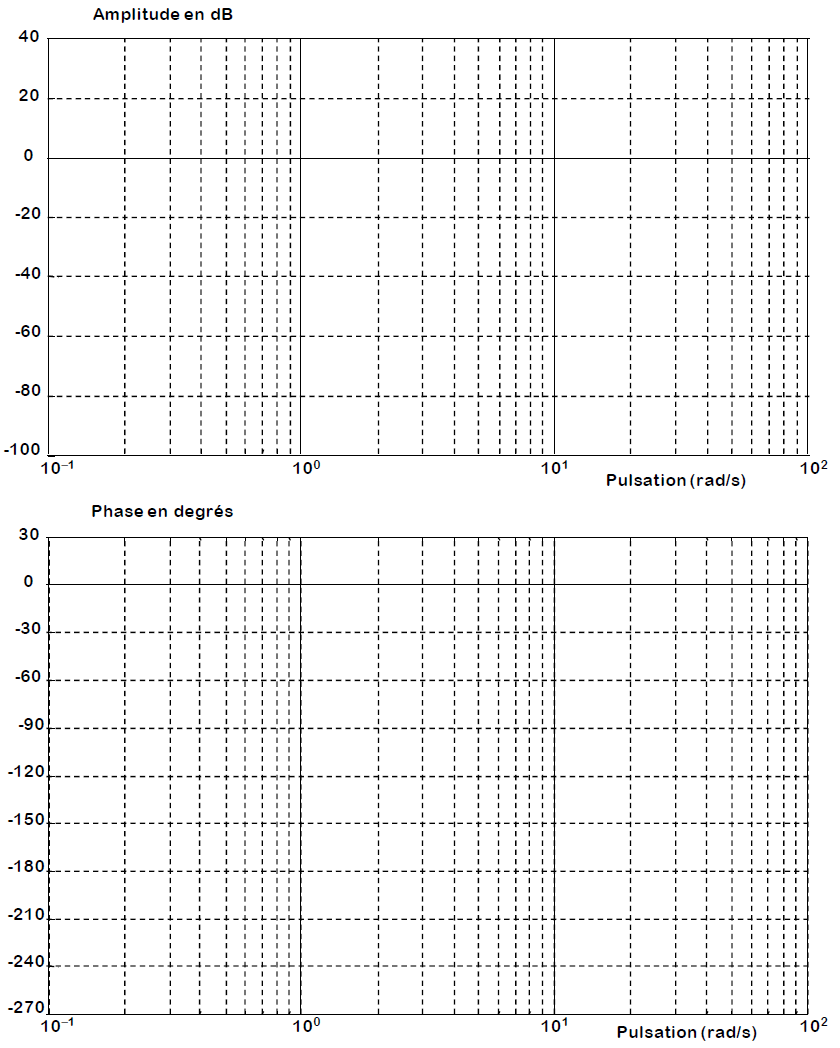
\includegraphics[width=0.8\linewidth]{img/DR01}
\end{center}

\reponse{23}{9}

\reponse{24}{11}

\reponse{25}{20}

\newpage

\reponse{26}{2}

\begin{center}
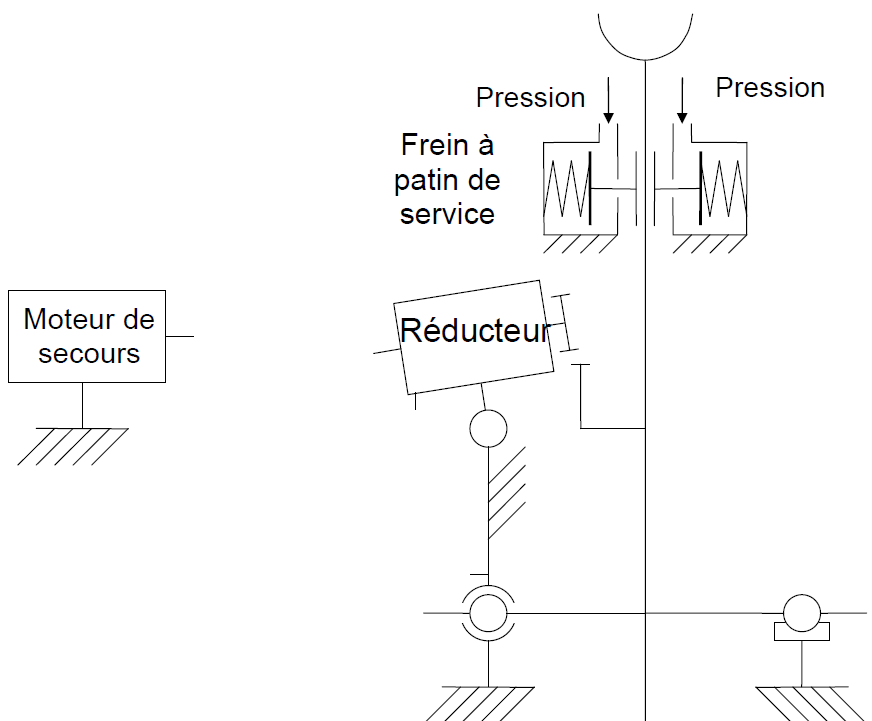
\includegraphics[width=0.8\linewidth]{img/DR02}
\end{center}

\newpage

\reponse{27}{2}

\begin{center}
\includegraphics[width=1.3\linewidth,angle=90]{img/Dessin01}
\end{center}

%\ifdef{\public}{\end{document}}{}

%\newpage
%\cleardoublepage

%\pagestyle{correction}

%\section{Correction}

\end{document}
